%%% LaTeX Template: Two column article
%%%
%%% Source: http://www.howtotex.com/
%%% Feel free to distribute this template, but please keep to referal to http://www.howtotex.com/ here.
%%% Date: February 2011

%%% Preamble
\documentclass[	DIV=calc,%
				paper=a4,%
				fontsize=9pt,%
				%onecolumn]{scrartcl}	 					% KOMA-article class
				onecolumn]{scrreprt}	 					% KOMA-article class
				%onecolumn]{report}	 					% KOMA-article class

\usepackage{lipsum}													% Package to create dummy text



\usepackage[english]{babel}										% English language/hyphenation
\usepackage[utf8]{inputenc}										% UTF-8 as input-encoding
\usepackage[protrusion=true,expansion=true]{microtype}				% Better typography
\usepackage{amsmath,amsfonts,amsthm}					% Math packages
\usepackage[pdftex]{graphicx}						% Enable pdflatex 
%\usepackage[svgnames]{xcolor}									% Enabling colors by their 'svgnames'
\usepackage[hang, small,labelfont=bf,up,textfont=it,up]{caption}	% Custom captions under/above floats
\usepackage{epstopdf}												% Converts .eps to .pdf
\usepackage{subfig}													% Subfigures
\usepackage{fix-cm}													% Custom fontsizes

\usepackage[usenames,dvipsnames]{color}
\usepackage{float}
\usepackage{subfig}
%\usepackage{tikz}
\usepackage{acronym}
\usepackage{amsthm}
\usepackage{fancyvrb}
\usepackage{upquote}												% For correct single quotes in listings
\usepackage{listings}
\usepackage{longtable}

%% Epigraph patching
\usepackage{epigraph}
% \epigraphsize{\small}% Default
\setlength\epigraphwidth{8cm}
\setlength\epigraphrule{0pt}
\usepackage{etoolbox}
\makeatletter
\patchcmd{\epigraph}{\@epitext{#1}}{\itshape\@epitext{#1}}{}{}
\makeatother



\usepackage{gitinfo}

% custom changes:
\usepackage[usenames,dvipsnames,svgnames,table]{xcolor}
\usepackage{placeins}
\usepackage{draftwatermark}

% human tables
\usepackage{booktabs}
\renewcommand{\arraystretch}{1.25}

% side box
\usepackage{wrapfig}
%\usepackage{tcolorbox}
\newenvironment{WrapText}[1][r]
  {\wrapfigure{#1}{0.5\textwidth}\tcolorbox}
  {\endtcolorbox\endwrapfigure}

% Add text symbols
\usepackage{pifont}
\newcommand{\yes}{\textcolor{green}{\ding{51}}}
\newcommand{\no}{\textcolor{red}{\ding{55}}}


% Colours
\definecolor{green}{RGB}{32,113,10}
\definecolor{orange}{RGB}{251,111,16}
\definecolor{red}{RGB}{247,56,0}
\definecolor{blue}{RGB}{0,28,128}
\definecolor{lightgreen}{RGB}{187,218,216}
\definecolor{intersectgreen}{RGB}{103,133,155}
\definecolor{darkblue}{RGB}{76,87,117}

\bibliographystyle{alphalink}

\definecolor{Brown}{cmyk}{0,0.81,1,0.60}
\definecolor{OliveGreen}{cmyk}{0.64,0,0.95,0.40}
\definecolor{CadetBlue}{cmyk}{0.62,0.57,0.23,0}
\definecolor{lightlightgray}{gray}{0.9}

\usepackage{titlesec}
%\allsectionsfont{\color{darkblue}\itshape\underline}
%\sectionfont{\color{darkblue}\itshape\selectfont}
%\subsectionfont{\color{darkblue}\itshape\selectfont}
\renewcommand*\sectfont{\sffamily\color{darkblue}\mdseries}
%\renewcommand*\sectfont{\rmfamily\mdseries\itshape}


% makes default font sans-serif
 \renewcommand{\familydefault}{\sfdefault}

% make font Open Sans
% \usepackage{opensans}
\usepackage[defaultsans]{opensans}

% changes font encoding to T1
% \usepackage[T1]{fontenc}
% \usepackage{textcomp}

% This block is for listings
\usepackage[framemethod=TikZ]{mdframed} % mdframed is used to draw a grey box
\mdfdefinestyle{listingstyle}{
  backgroundcolor=black!10,outerlinewidth=0,outerlinecolor=black,
  innerleftmargin=0,innerrightmargin=0,innertopmargin=0pt,innerbottommargin=0pt
}
\usepackage{amssymb}% for \curvearrowright
% Insert a grey box behind the listing for uniform background color (The \cipherstring would the listing and the background would turn white)
\BeforeBeginEnvironment{lstlisting}{\vspace{0.2cm}\begin{mdframed}[style=listingstyle]}
\AfterEndEnvironment{lstlisting}{\end{mdframed}}
\lstset{
%language=Bash,                             % Code langugage
basicstyle=\ttfamily,                   % Code font, Examples: \footnotesize, \ttfamily
keywordstyle=\color{OliveGreen},        % Keywords font ('*' = uppercase)
commentstyle=\color{gray},              % Comments font
%numbers=left,                           % Line nums position
%numberstyle=\tiny,                      % Line-numbers fonts
%stepnumber=1,                           % Step between two line-numbers
%numbersep=5pt,                          % How far are line-numbers from code
backgroundcolor=\color{lightlightgray}, % Choose background color
frame=none,                             % A frame around the code
tabsize=2,                              % Default tab size
captionpos=b,                           % Caption-position = bottom
breaklines=true,                        % Automatic line breaking?
breakatwhitespace=false,                % Automatic breaks only at whitespace?
showspaces=false,                       % Dont make spaces visible
showstringspaces=false,
showtabs=false,                         % Dont make tabls visible
columns=fullflexible,                   % Column format: no spaces are inserted for monospaced appearance
morekeywords={__global__, __device__},  % 
escapeinside={\%*}{*)},                 % Escape TeX commands inside %* and *)
prebreak=\mbox{$\curvearrowright$},     % Disply curved arrow before linebreak
xrightmargin=1.8pt,
}


%% \todo{} command.
%
% Outputs red TODOs in the document. Requires \usepackage{color}.
%
% Usage: \todo{Document the TODO command.}
%
% Comment out second line to disable.
\newcommand{\todo}[1]{}
\renewcommand{\todo}[1]{{\color{Red} TODO: {#1}}}


%%% Custom sectioning (sectsty package)
\usepackage{sectsty}													% Custom sectioning (see below)
\allsectionsfont{%															% Change font of al section commands
	%\usefont{OT1}{phv}{b}{n}%										% bch-b-n: CharterBT-Bold font 
\bfseries 															% should make it Open Sans Bold
	}

\sectionfont{%																% Change font of \section command
	%\usefont{OT1}{phv}{b}{n}%										% bch-b-n: CharterBT-Bold font
\bfseries 	
	}

% use more of the page
\usepackage{fullpage}

%%% Headers and footers
\usepackage{fancyhdr}												% Needed to define custom headers/footers
	\pagestyle{fancy}														% Enabling the custom headers/footers
\usepackage{lastpage}	

% Header (empty)
\lhead{}
\chead{}
\rhead{}
% Footer (you may change this to your own needs)
\lfoot{\footnotesize Applied Crypto Hardening \textbullet ~Draft revision\gitVtags: \gitAbbrevHash{} (\gitCommitterIsoDate) \gitCommitterName}
\cfoot{}
\rfoot{\footnotesize page \thepage\ of \pageref{LastPage}}	% "Page 1 of 2"
\renewcommand{\headrulewidth}{0.0pt}
\renewcommand{\footrulewidth}{0.4pt}



%%% Creating an initial of the very first character of the content
\usepackage{lettrine}
\newcommand{\initial}[1]{%
     \lettrine[lines=3,lhang=0.3,nindent=0em]{
     				\color{darkblue}
     				{\textsf{#1}}}{}}



%%% Title, author and date metadata
\usepackage{titling}															% For custom titles

\newcommand{\HorRule}{\color{darkblue}%			% Creating a horizontal rule
									  	\rule{\linewidth}{1pt}%
									}


\pretitle{\vspace{-30pt} \begin{flushleft} \HorRule 
				\fontsize{35}{36} \bfseries \color{darkblue} \selectfont 
				}
			\title{Applied Crypto Hardening}% \\ \vskip 0.5em \large www.bettercrypto.org}
\posttitle{\par\end{flushleft}\vskip 0.5em}

\preauthor{\begin{flushleft}
					\large \lineskip 0.5em  
					\color{intersectgreen}}
					%\vskip 0.5em
					\author{Wolfgang Breyha, David Durvaux, Tobias Dussa, L. Aaron
					Kaplan, Florian Mendel, Christian Mock, Manuel Koschuch, Adi
					Kriegisch, Ulrich Pöschl, Ramin Sabet, Berg San, Ralf Schlatterbeck, 
					Thomas Schreck, Aaron Zauner, Pepi Zawodsky}
%\institute{
%FH Campus Wien
%\and
%VRVis
%\and
%CERT.at
%\and
%Karlsruhe Institute of Technology
%}


\setlength{\parindent}{0cm}

\postauthor{\footnotesize  \color{Black}  \vskip 2.5em
  (University of Vienna, CERT.be, KIT-CERT, CERT.at, IAIK, coretec.at, FH Campus Wien, VRVis, MilCERT Austria, A-Trust, Runtux.com, Friedrich-Alexander University Erlangen-Nuremberg, azet.org, maclemon.at)
					\par\end{flushleft}\HorRule}

\date{\today}

%tell TeX where to look for graphics/logos
\graphicspath{ {/img/} }

% hyperref needs to be the last package you load.
\usepackage[pdftex,breaklinks,colorlinks,linkcolor=darkblue,citecolor=blue,urlcolor=blue]{hyperref}

% CIPHERSTRING
\usepackage{seqsplit} % Use Sequence split. Basically it inserts between every character pair a box with zero width to allow linebreaks everywhere. Better solution wanted, but is there any better?
\newcommand{\cipherstringB}{\seqsplit{EDH+CAMELLIA:EDH+aRSA:EECDH+aRSA+AESGCM:EECDH+aRSA+SHA384:EECDH+aRSA+SHA256:EECDH:+CAMELLIA256:+AES256:+CAMELLIA128:+AES128:+SSLv3:!aNULL:!eNULL:!LOW:!3DES:!MD5:!EXP:!PSK:!SRP:!DSS:!RC4:!SEED:!ECDSA:CAMELLIA256-SHA:AES256-SHA:CAMELLIA128-SHA:AES128-SHA}}

%%% Begin document
\begin{document}
\maketitle

\thispagestyle{fancy} 			% Enabling the custom headers/footers for the first page 
% The first character should be within \initial{}
%\initial{H}\textbf{ere is some sample text to show the initial in the introductory paragraph of this template article. The color and lineheight of the initial can be modified in the preamble of this document.}

% add logo graphic
%
\includegraphics{img/logo}

% move this epigraph to a fitting place. I don't see why it fits here inside of the begin figure env. ~~ AK
%\epigraph{``[...] be conservative in what you do, be liberal in what
%you accept from others.''}{The robustness priciple or ``Postel's Law''~\cite{rfc761}}
{\centering
  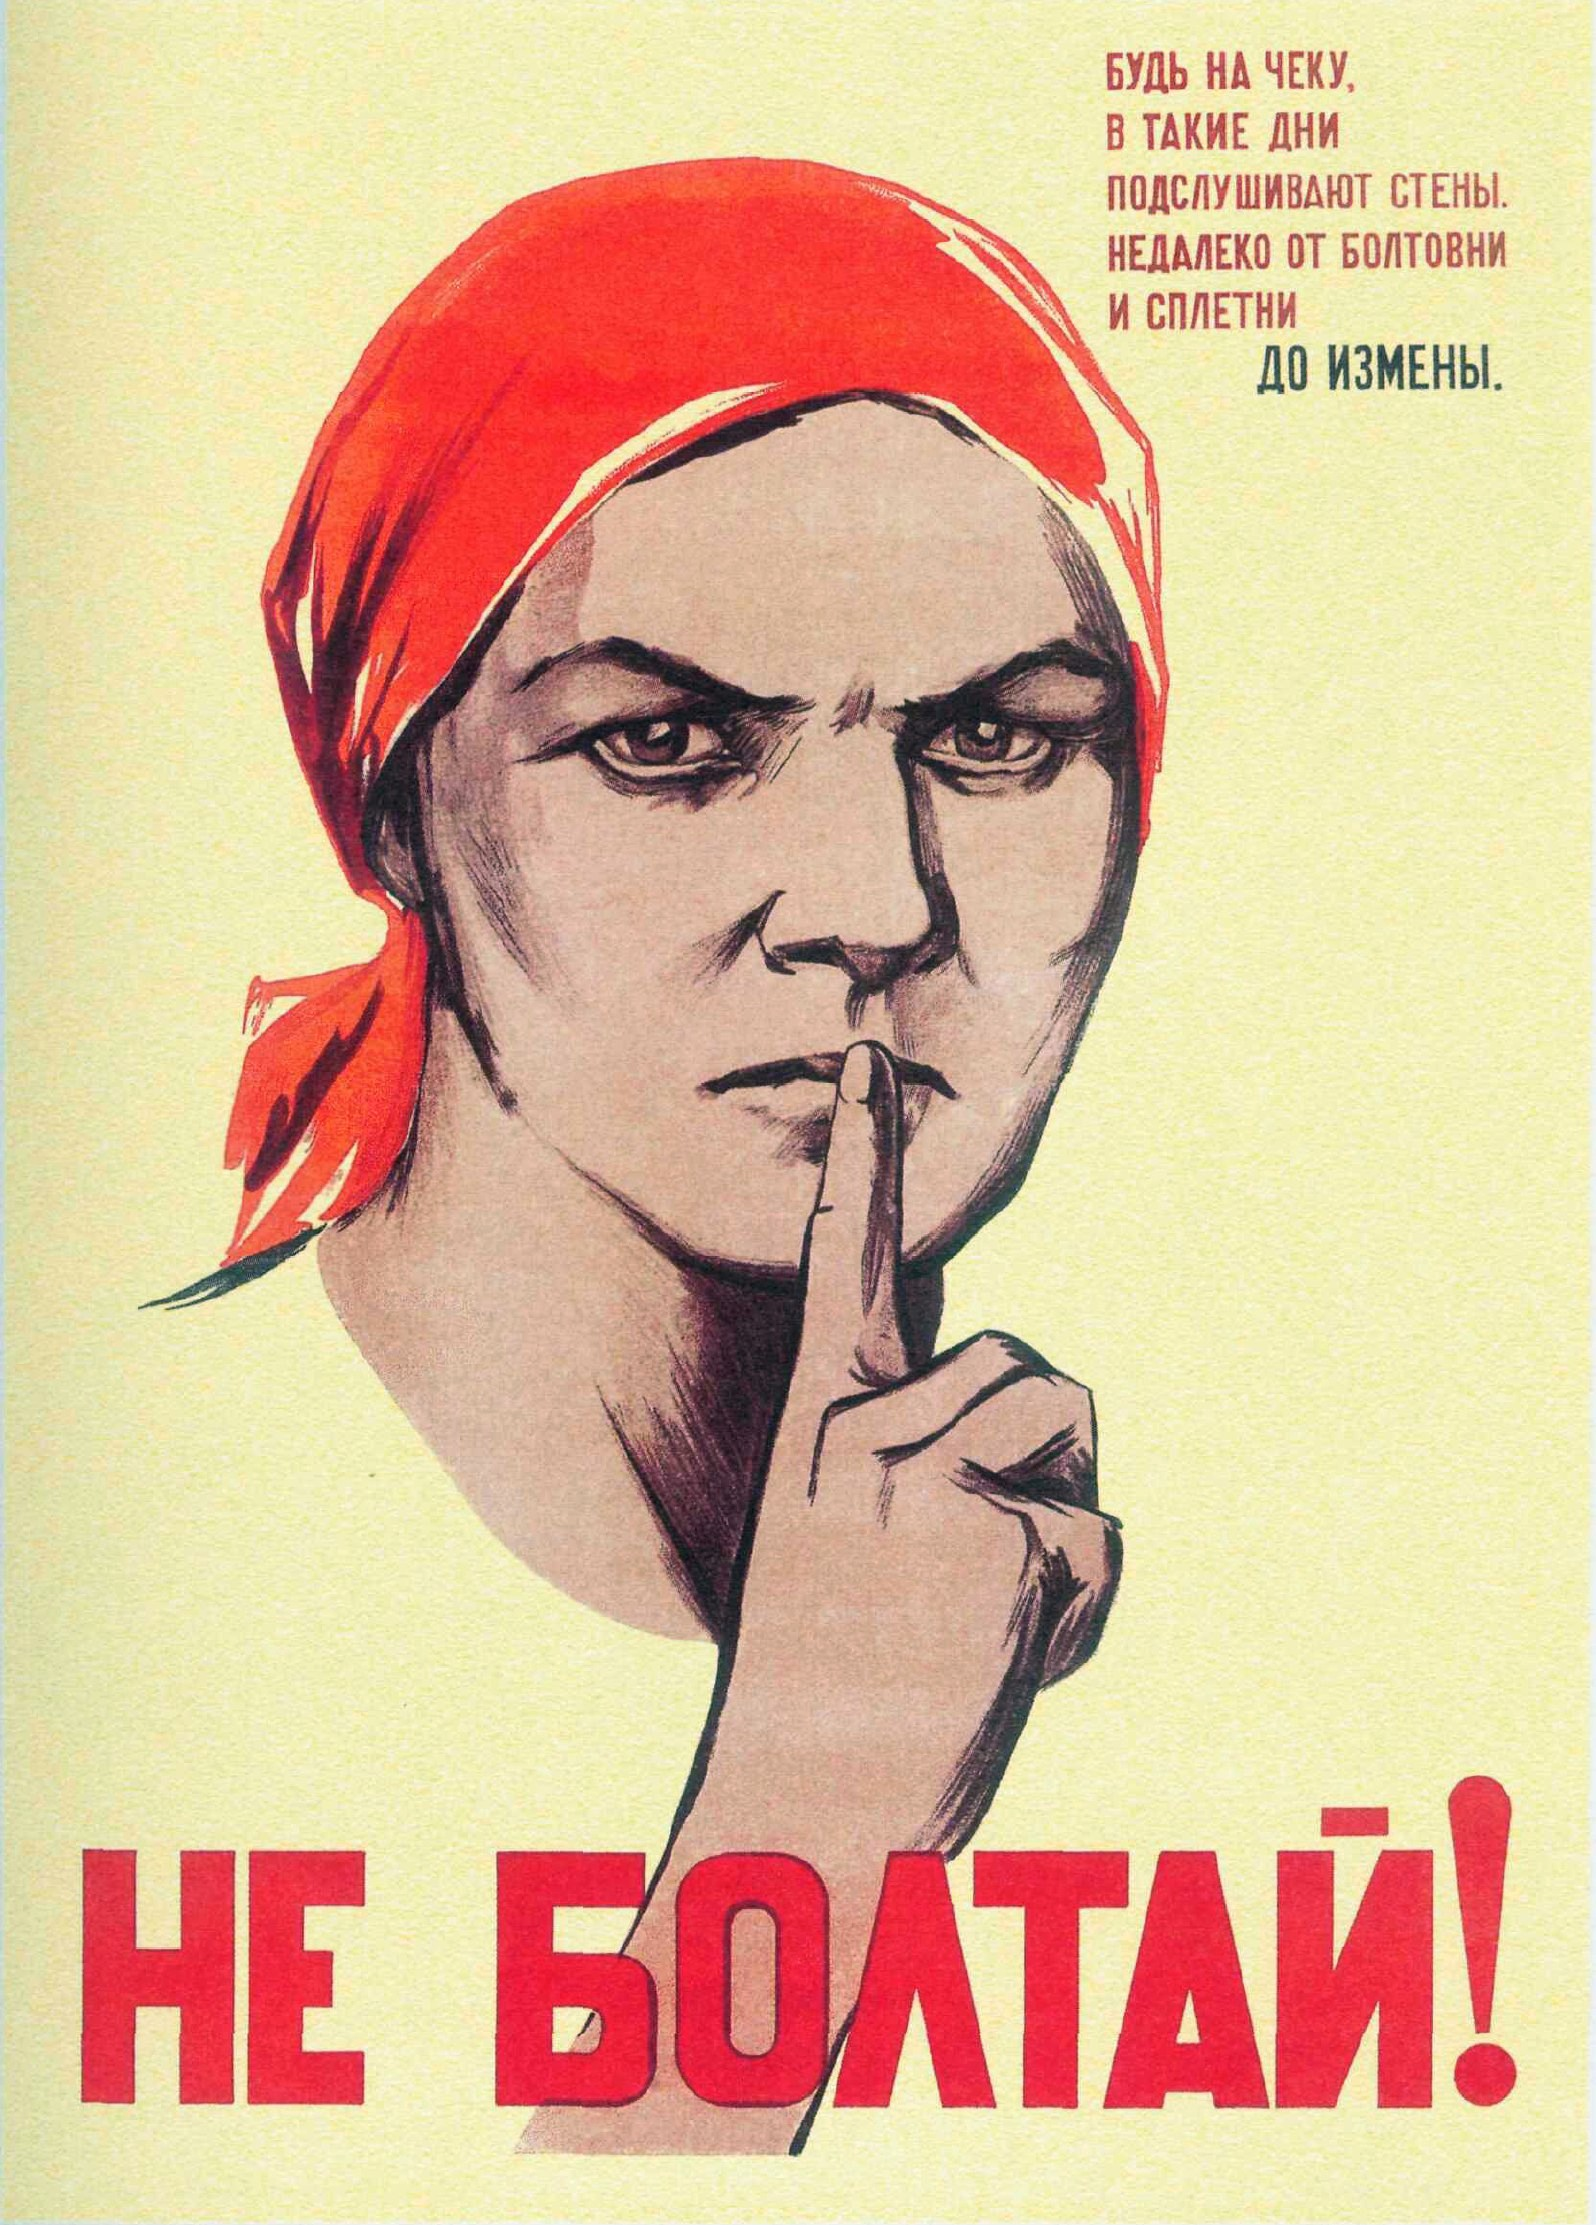
\includegraphics[width=.9\textwidth]{neboltai.jpg}\par
  \vbox{\emph{Do not talk unencrypted}}
}
%%% Local Variables: 
%%% mode: latex
%%% TeX-master: "applied-crypto-hardening"
%%% End: 

\clearpage
\section*{Acknowledgements}
\label{section:Reviewers}

We would like to express our thanks to the following reviewers and people who have generously offered their time and interest (in alphabetical order):

\begin{multicols}{2}{\parskip=0pt\centering\obeylines%
Brown, Scott \\
Brulebois, Cyril \\
Delmas, Tom \\
Dirksen-Thedens, Mathis \\
Dulaunoy, Alexandre \\
Gühring Philipp  \\
Grigg, Ian  \\
Horenbeck, Maarten \\
Huebl, Axel \\
Kovacic, Daniel \\
Lenzhofer, Stefan \\
Lorünser, Thomas \\
Mehlmauer, Christian \\
Millauer, Tobias \\
Mirbach, Andreas \\
O'Brien, Hugh \\
Pacher, Christoph \\
Palfrader, Peter \\
Pape, Tobias (layout) \\
Petukhova, Anna (Logo) \\
Pichler, Patrick \\
Riebesel, Nicolas \\
Roeckx, Kurt \\
Roesen, Jens \\
Rublik, Martin \\
Schüpany, Mathias \\
Schwarz, René («DigNative») \\
Seidl, Eva (PDF layout) \\
Wagner, Sebastian («sebix») \\
Zangerl, Alexander \\
}\end{multicols}


%% *@discuss@lists.cert.at --> AKA
%% devops mailing lists --> Pepi, Azet
%% cryptography liste (at release time) --> Azet



The reviewers did review parts of the document in their area of
expertise; all remaining errors in this document are the sole
responsibility of the primary authors.

%% *@discuss@lists.cert.at --> AKA
%% devops mailing lists --> Pepi, Azet
%% cryptography liste (at release time) --> Azet



%%% Local Variables:
%%% mode: latex
%%% TeX-master: "applied-crypto-hardening"
%%% End:

\input{abstract}
\tableofcontents
\chapter{Introduction}
\label{chapter:Intro}
\input{whoshouldread}
\input{related_publications}
\section{How to read this guide}
\label{sec:how-read-this}
This guide tries to accommodate two needs: first of all, having a handy reference on how to configure the most common services' crypto settings and second of all, explain a bit of background on cryptography. This background is essential if the reader wants to choose his or her own cipher string settings.

System administrators who want to copy \& paste recommendations quickly without
spending a lot of time on background reading on cryptography or cryptanalysis
can do so, by simply searching for the corresponding section in chapter
\ref{chapter:PracticalSettings} (``Practical recommendations'').

It is important to know that in this guide the authors arrived at two recommendations: \textit{Cipher string A} and \textit{Cipher string B}. While the former is a hardened recommendation the latter is a weaker one but provides wider compatibility.
\textit{Cipher strings A and B} are described in \ref{section:recommendedciphers}.

%\textit{Cipher
%string B} covers the most common use-cases (such as running an e-commerce shop,
%a private homepage, a mail server, $ \ldots $).

However, for the quick copy \& paste approach it is important to know that this
guide assumes users are happy with \textit{Cipher string B}.


While chapter \ref{chapter:PracticalSettings} is intended to serve as a copy \& paste reference, chapter \ref{chapter:Theory} (``Theory'') explains the reasoning behind \textit{cipher string B}. In particular, section \ref{section:CipherSuites} explains how to choose individual cipher strings. We advise the reader to actually read this section and challenge our reasoning in choosing \textit{Cipher string B} and to come up with a better  or localized solution.

%We start with some general remarks in sections \ref{section:DH},\ref{section:EllipticCurveCryptography},\ref{section:keylengths} on 
%If you are a system administrator and want to quickly update your services, jump right to section \ref{section:PracticalSettings}. However, we recommend that you take some time and first read through the theory part (chapter \ref{chapter:Theory}), especially section \ref{section:CipherSuites} on how to choose your own cipher string and then adapt the settings in section \ref{section:PracticalSettings} to your own needs.

\tikzstyle{terminator} = [ellipse, draw,  minimum height=2em,
    text width=4.5em, text badly centered, inner sep=0pt]
\tikzstyle{decision} = [diamond, draw,aspect=2,
     text width=10em, text badly centered, node distance=8em, inner sep=0pt]
\tikzstyle{block} = [rectangle, draw,inner sep=0pt,
     text width=17em, text centered, rounded corners, minimum height=4em]
\tikzstyle{line} = [draw, very thick, -latex']
\tikzstyle{decision answer}=[near start,color=black]
\begin{tikzpicture}[scale=1, node distance = 6em, auto]
    % Place nodes
    \node [terminator] (start) {Start};
    \node [block, right of=start, text width=7em, node distance=8em] (intro) {%
      \nameref{chapter:Intro}};
    \node [decision, below of=intro] (evaluate) {%
      No time, I just want to copy \& paste};
    \node [block, right of=evaluate, node distance=20em] (practical1) {%
      read \nameref{chapter:PracticalSettings}};
    \node [block, below of=evaluate,node distance=8em ] (theory) {%
      To understand why we chose certain settings, read
      \nameref{chapter:Theory} first};
    \node [block, right of=theory, node distance=20em] (practical2) {%
      re-read \nameref{chapter:PracticalSettings}};
    \node [block, below of =practical2] (appendix) {%
      \hyperref[appendix]{Appendix}: references, links};
    % Draw edges
    \path [line] (start) -- (intro);
    \path [line] (intro) -- (evaluate);
    \path [line] (evaluate) -- node [decision answer]  {yes} (practical1);
    \path [line] (evaluate) -- node [decision answer]  {no} (theory);
    \path [line] (practical1) -- (theory);
    \path [line] (theory) -- (practical2);
    \path [line] (practical2) -- (appendix);
\end{tikzpicture}

%%% Local Variables: 
%%% mode: latex
%%% TeX-master: "applied-crypto-hardening"
%%% End: 

\newpage
\section{Disclaimer and scope}
\label{section:disclaimer}

\epigraph{``A chain is no stronger than its weakest link, and life is after all a chain''}{-- William James}

\epigraph{``Encryption works. Properly implemented strong crypto systems are
one of the few things that you can rely on. Unfortunately, endpoint security is
so terrifically weak that NSA can frequently find ways around it.''}{--- Edward
Snowden, answering questions live on the Guardian's
website\cite{snowdenGuardianGreenwald}}


This guide specifically does not address physical security, protecting software
and hardware against exploits, basic IT security housekeeping, information
assurance techniques, traffic analysis attacks, issues with key-roll over and
key management, securing client PCs and mobile devices (theft, loss), proper
OPSec\footnote{\url{http://en.wikipedia.org/wiki/Operations_security}}, social
engineering attacks, anti-tempest\cite{Wikipedia:Tempest} attack techniques,
protecting against different side-channel attacks (timing--, cache timing--,
differential fault analysis, differential power analysis or power monitoring
attacks), downgrade attacks, jamming the encrypted channel or other similar
attacks which are typically employed to circumvent strong encryption.  The
authors can not overstate the importance of these other techniques.  Interested
readers are advised to read about these attacks in detail since they give a lot
of insight into other parts of cryptography engineering which need to be dealt
with.\footnote{An easy to read yet very insightful recent example is the
"FLUSH+RELOAD" technique \cite{yarom2013flush+} for leaking cryptographic keys
from one virtual machine to another via L3 cache timing attacks.}

\vskip 0.5em
This guide does not talk much about the well-known insecurities of trusting a
public-key infrastructure (PKI)\footnote{Interested readers are referred to
\url{https://bugzilla.mozilla.org/show_bug.cgi?id=647959} or
\url{http://www.heise.de/security/meldung/Der-ehrliche-Achmed-bittet-um-Vertrauen-1231083.html}
(german) which brings the problem of trusting PKIs right to the point}. Nor
does this text fully explain how to run your own Certificate Authority (CA). 


\vskip 0.5em
Most of this zoo of information security issues are addressed in the very
comprehensive book ``Security Engineering'' by Ross Anderson
\cite{anderson2008security}. 

For some experts in cryptography this text might seem too informal. However, we
strive to keep the language as non-technical as possible and fitting for our
target audience: system administrators who can collectively improve the
security level for all of their users. 

\vskip 0.5em


\epigraph{``Security is a process, not a product.''}{-- Bruce Schneier}

This guide can only describe what the authors currently
\emph{believe} to be the best settings based on their personal experience and
after intensive cross checking with literature and experts. For a complete list
of people who reviewed this paper, see the section \ref{section:Reviewers}.
Even though multiple specialists reviewed the guide, the authors can give
\emph{no guarantee whatsoever} that they made the right recommendations. Keep in
mind that tomorrow there might be new attacks on some ciphers and many of the
recommendations in this guide might turn out to be wrong. Security is a
process.

\vskip 0.5em

We therefore recommend that system administrators keep up to date with recent
topics in IT security and cryptography. 


In this sense, this guide is very focused on getting the cipher strings done
right even though there is much more to do in order to make a system more
secure.  We the authors, need this document as much as the reader needs it.

\paragraph{Scope:}
\label{section:Scope}

In this guide, we restricted ourselves to:
\begin{itemize}
\item Internet-facing services
\item Commonly used services
\item Devices which are used in business environments (this specifically excludes XBoxes, Playstations and similar consumer devices)
\item OpenSSL 
\end{itemize}

We explicitly excluded:
\begin{itemize}
\item Specialized systems (such as medical devices, most embedded systems, etc.)
\item Wireless Access Points
\item Smart-cards/chip cards
%\item Advice on running a PKI or a CA
%\item Services which should be run only in an internal network and never face the Internet.
\end{itemize}


\input{motivation}
\input{methods}
%%
\chapter{Practical recommendations}
\label{chapter:PracticalSettings}
\section{Webservers}
\label{sec:webservers}
%%\subsection{Webservers}

%%---------------------------------------------------------------------- 
\subsection{Apache}

\subsubsection{Tested with Versions} 
\begin{itemize}
\item Apache 2.4.6 linked against OpenSSL 1.0.1e, Debian jessie
\end{itemize}


\subsubsection{Settings} 

Enabled modules \emph{SSL} and \emph{Headers} are required.

%-All +TLSv1.1 +TLSv1.2
\begin{lstlisting}[breaklines]
  SSLCertificateFile server.crt
  SSLCertificateKeyFile server.key
  SSLProtocol All -SSLv2 -SSLv3 
  SSLHonorCipherOrder On
  SSLCompression off
  # Add six earth month HSTS header for all users...
  Header add Strict-Transport-Security "max-age=15768000"
  # If you want to protect all subdomains, use the following header
  # ALL subdomains HAVE TO support https if you use this!
  # Strict-Transport-Security: max-age=15768000 ; includeSubDomains

  SSLCipherSuite '@@@CIPHERSTRINGB@@@'

\end{lstlisting}

Note that any cipher suite starting with EECDH can be omitted, if in doubt.
(Compared to the theory section, EECDH in Apache and ECDHE in OpenSSL are
synonyms~\footnote{https://www.mail-archive.com/openssl-dev@openssl.org/msg33405.html})

\subsubsection{Additional settings}

You might want to redirect everything to http\textbf{s}:// if possible. In Apache you can do this with the following setting inside of a VirtualHost environment:

\begin{lstlisting}[breaklines]
  <VirtualHost *:80>
   #...
   RewriteEngine On
        RewriteRule ^.*$ https://%{SERVER_NAME}%{REQUEST_URI} [L,R=permanent]
   #...
  </VirtualHost>
\end{lstlisting}

%\subsubsection{Justification for special settings (if needed)}

\subsubsection{References}
\url{https://httpd.apache.org/docs/2.4/ssl/}


\subsubsection{How to test}

See appendix \ref{cha:tools}

%%\end{description}


%%---------------------------------------------------------------------- 
\subsection{lighttpd}



%%\begin{description}
\subsubsection{Tested with Version}
\begin{itemize}
\item lighttpd/1.4.31-4 with OpenSSL 1.0.1e on Debian 7.0
\item lighttpd/1.4.33 with OpenSSL 0.9.8o on Debian Squeeze (note that TLSv1.2 does not work in openssl 0.9.8 thus not all ciphers actually work)
\item lighttpd/1.4.28-2 with OpenSSL 0.9.8o on Debian Squeeze (note that TLSv1.2 does not work in openssl 0.9.8 thus not all ciphers actually work)
\end{itemize}


\subsubsection{Settings}


%% Complete ssl.cipher-list with same algo than Apache
\todo{FIXME: this string seems to be wrongly formatted??}

\begin{lstlisting}[breaklines]
  $SERVER["socket"] == "0.0.0.0:443" {
    ssl.engine  = "enable"
    ssl.use-sslv2 = "disable"
    ssl.use-sslv3 = "disable"
    #ssl.use-compression obsolete >= 1.4.3.1
    ssl.pemfile = "/etc/lighttpd/server.pem"
    ssl.cipher-list = "@@@CIPHERSTRINGB@@@"
    ssl.honor-cipher-order = "enable"
    setenv.add-response-header  = ( "Strict-Transport-Security" => "max-age=31536000")
  }
\end{lstlisting}


\subsubsection{Additional settings}

As for any other webserver, you might want to automatically redirect http
traffic toward http\textbf{s}:// It is also recommended to set the environment variable
\emph{HTTPS}, so the applications run by the webserver can easily detect, that
HTTPS is in use.



\begin{lstlisting}[breaklines]
  $HTTP["scheme"] == "http" {
    # capture vhost name with regex conditiona -> %0 in redirect pattern
    # must be the most inner block to the redirect rule
    $HTTP["host"] =~ ".*" {
        url.redirect = (".*" => "https://%0$0")
    }
  # Set the environment variable properly
  setenv.add-environment = (
            "HTTPS" => "on"
        )
  }
\end{lstlisting}


\subsubsection{Additional information} 
The config option \emph{honor-cipher-order} is available since 1.4.30, the
supported ciphers depend on the used OpenSSL-version (at runtime). ECDH has to
be available in OpenSSL at compile-time, which should be default. SSL
compression should by deactivated by default at compile-time (if not, it's
active).

Support for other SSL-libraries like GnuTLS will be available in the upcoming
2.x branch, which is currently under development.


\subsubsection{References} 

\begin{itemize}
        \item HTTPS redirection: \url{http://redmine.lighttpd.net/projects/1/wiki/HowToRedirectHttpToHttps}
        \item Lighttpd Docs SSL: \url{http://redmine.lighttpd.net/projects/lighttpd/wiki/Docs\_SSL}
        \item Release 1.4.30 (How to mitigate BEAST attack) \url{http://redmine.lighttpd.net/projects/lighttpd/wiki/Release-1\_4\_30}
        \item SSL Compression disabled by default: \url{http://redmine.lighttpd.net/issues/2445}
\end{itemize}




\subsubsection{How to test} 
See appendix \ref{cha:tools}



%%---------------------------------------------------------------------- 
\subsection{nginx}

%\begin{description}
\subsubsection{Tested with Version} 
\begin{itemize}
\item 1.4.4 with OpenSSL 1.0.1e on OS X Server 10.8.5
\item 1.2.1-2.2+wheezy2 with OpenSSL 1.0.1e on Debian 7.0
\item 1.4.4 with OpenSSL 1.0.1e on Debian 7.0
\item 1.2.1-2.2~bpo60+2 with OpenSSL 0.9.8o on Debian Squeeze (note that TLSv1.2 does not work in openssl 0.9.8 thus not all ciphers actually work)
\end{itemize}


\subsubsection{Settings}

\begin{lstlisting}[breaklines]
  ssl_prefer_server_ciphers on;
  ssl_protocols TLSv1 TLSv1.1 TLSv1.2; # not possible to do exclusive
  ssl_ciphers '@@@CIPHERSTRINGB@@@';
  add_header Strict-Transport-Security max-age=2592000;
\end{lstlisting}

If you absolutely want to specify your own DH parameters, you can specify them via

\begin{lstlisting}[breaklines]
  ssl_dhparam file;
\end{lstlisting}

However, we advise you to read section \ref{section:DH} and stay with the standard IKE/IETF parameters (as long as they are $ > 1024 $ bits).

\subsubsection{Additional settings}

If you decide to trust NIST's ECC curve recommendation, you can add the following line to nginx's configuration file to select special curves:

\begin{lstlisting}[breaklines]
  ssl_ecdh_curve          secp384r1;
\end{lstlisting}

You might want to redirect everything to http\textbf{s}:// if possible. In Nginx you can do this with the following setting:

\begin{lstlisting}[breaklines]
  return 301 https://$host$request_uri;
\end{lstlisting}


\subsubsection{References} 
\begin{itemize}
\item \url{http://nginx.org/en/docs/http/ngx_http_ssl_module.html}
\item \url{http://wiki.nginx.org/HttpSslModule}
\end{itemize}

\subsubsection{How to test}
See appendix \ref{cha:tools}





%%---------------------------------------------------------------------- 
\subsection{MS IIS}
\label{sec:ms-iis}

To configure SSL/TLS on Windows Server you can use IIS Crypto~\footnote{\url{https://www.nartac.com/Products/IISCrypto/}}
Simply start the Programm no installation required. The tool changes the registry keys described below.
A restart ist required for the changes to take effect.

\todo add iis crypto screenshot here

Instead of using the IIS Crypto Tool the configuration can be set
using the Windows Registry. The following Registry keys apply to the
newer Versions of Windows (Windows 7, Windows Server 2008, Windows
Server 2008 R2, Windows Server 2012 and Windows Server 2012 R2). For detailed
information about the older versions see the Microsoft knowlagebase
article. \footnote{\url{http://support.microsoft.com/kb/245030/en-us}}
\begin{lstlisting}[breaklines]
  [HKEY_LOCAL_MACHINE\SYSTEM\CurrentControlSet\Control\SecurityProviders\Schannel] 
  [HKEY_LOCAL_MACHINE\SYSTEM\CurrentControlSet\Control\SecurityProviders\Schannel\Ciphers] 
  [HKEY_LOCAL_MACHINE\SYSTEM\CurrentControlSet\Control\SecurityProviders\Schannel\CipherSuites] 
  [HKEY_LOCAL_MACHINE\SYSTEM\CurrentControlSet\Control\SecurityProviders\Schannel\Hashes] 
  [HKEY_LOCAL_MACHINE\SYSTEM\CurrentControlSet\Control\SecurityProviders\Schannel\KeyExchangeAlgorithms] 
  [HKEY_LOCAL_MACHINE\SYSTEM\CurrentControlSet\Control\SecurityProviders\Schannel\Protocols] 
\end{lstlisting}

Windows Server 2008 and Windows XP supports the following protocols:
\begin{itemize}
\item SSL 2.0
\item SSL 3.0
\item TLS 1.0
\end{itemize}

Windows Server 2008 R2 and newer and Windows 7 and newer support the following protocols:
\begin{itemize}
\item SSL 2.0
\item SSL 3.0
\item TLS 1.0
\item TLS 1.1
\item TLS 1.2
\end{itemize}

The srandard chipher order for TLS1.0 of Windows Server 2003 and Windows XP
\begin{itemize}
\item TLS_RSA_WITH_RC4_128_MD5
\item TLS_RSA_WITH_RC4_128_SHA
\item TLS_RSA_WITH_3DES_EDE_CBC_SHA
\item TLS_DHE_DSS_WITH_3DES_EDE_CBC_SHA
\item TLS_RSA_WITH_DES_CBC_SHA
\item TLS_DHE_DSS_WITH_DES_CBC_SHA
\item TLS_RSA_EXPORT1024_WITH_RC4_56_SHA
\item TLS_RSA_EXPORT1024_WITH_DES_CBC_SHA
\item TLS_DHE_DSS_EXPORT1024_WITH_DES_CBC_SHA
\item TLS_RSA_EXPORT_WITH_RC4_40_MD5
\item TLS_RSA_EXPORT_WITH_RC2_CBC_40_MD5
\item TLS_RSA_WITH_NULL_MD5
\item TLS_RSA_WITH_NULL_SHA
\end{itemize}

the standard chipher order in Windows 2008 and Windows Vista an above
\begin{table}[h]
  \centering
  \small
  \begin{tabular}{ll}
    \toprule
    Cipher suite	FIPS mode enabled	Exchange	Encryption	Hash	Protocols\\
    \midrule
\verb|TLS_RSA_WITH_AES_128_CBC_SHA|Yes|RSA|AES|SHA1|TLS 1.0\\
\verb|TLS_RSA_WITH_AES_256_CBC_SHA|Yes|RSA|AES|SHA1|TLS 1.0\\
\verb|TLS_RSA_WITH_RC4_128_SHA|No|RSA|RC4|SHA1|TLS 1.0, SSL 3.0\\
\verb|TLS_RSA_WITH_3DES_EDE_CBC_SHA|Yes|RSA|3DES|SHA1|TLS 1.0\\
\verb|TLS_ECDHE_ECDSA_WITH_AES_128_CBC_SHA_P256|Yes|ECDH_P256|AES|SHA1|TLS 1.0\\
\verb|TLS_ECDHE_ECDSA_WITH_AES_128_CBC_SHA_P384|Yes|ECDH_P384|AES|SHA1|TLS 1.0\\
\verb|TLS_ECDHE_ECDSA_WITH_AES_128_CBC_SHA_P521|Yes|ECDH_P521|AES|SHA1|TLS 1.0\\
\verb|TLS_ECDHE_ECDSA_WITH_AES_256_CBC_SHA_P256|Yes|ECDH_P256|AES|SHA1|TLS 1.0\\
\verb|TLS_ECDHE_ECDSA_WITH_AES_256_CBC_SHA_P384|Yes|ECDH_P384|AES|SHA1|TLS 1.0\\
\verb|TLS_ECDHE_ECDSA_WITH_AES_256_CBC_SHA_P521|Yes|ECDH_P521|AES|SHA1|TLS 1.0\\
\verb|TLS_ECDHE_RSA_WITH_AES_128_CBC_SHA_P256|Yes|ECDH_P256|AES|SHA1|TLS 1.0\\
\verb|TLS_ECDHE_RSA_WITH_AES_128_CBC_SHA_P384|Yes|ECDH_P384|AES|SHA1|TLS 1.0\\
\verb|TLS_ECDHE_RSA_WITH_AES_128_CBC_SHA_P521|Yes|ECDH_P521|AES|SHA1|TLS 1.0\\
\verb|TLS_ECDHE_RSA_WITH_AES_256_CBC_SHA_P256|Yes|ECDH_P256|AES|SHA1|TLS 1.0\\
\verb|TLS_ECDHE_RSA_WITH_AES_256_CBC_SHA_P384|Yes|ECDH_P384|AES|SHA1|TLS 1.0\\
\verb|TLS_ECDHE_RSA_WITH_AES_256_CBC_SHA_P521|Yes|ECDH_P521|AES|SHA1|TLS 1.0\\
\verb|TLS_DHE_DSS_WITH_AES_128_CBC_SHA|Yes|DH|AES|SHA1|TLS 1.0\\
\verb|TLS_DHE_DSS_WITH_AES_256_CBC_SHA|Yes|DH|AES|SHA1|TLS 1.0\\
\verb|TLS_DHE_DSS_WITH_3DES_EDE_CBC_SHA|Yes|DH|3DES|SHA1|TLS 1.0, SSL 3.0\\
\verb|TLS_RSA_WITH_RC4_128_MD5|No|RSA|RC4|MD5|TLS 1.0, SSL 3.0\\
\verb|SSL_CK_RC4_128_WITH_MD5|No|RSA|RC4|MD5|SSL 2.0\\
\verb|SSL_CK_DES_192_EDE3_CBC_WITH_MD5|No|RSA|3DES|MD5|SSL 2.0\\
\verb|TLS_RSA_WITH_NULL_MD5|No|RSA|MD5|TLS 1.0, SSL 3.0\\
\verb|TLS_RSA_WITH_NULL_SHA|No|RSA|SHA1|TLS 1.0, SSL 3.0\\
 \bottomrule 
 \end{tabular}
  \caption{Client support}
  \label{tab:MS_IIS_Client_Support}
\end{table}

%\begin{description}

\subsubsection{Tested with Version} \todo{Daniel: add tested version}

\begin{itemize}
\item Windows Server 2012 R2 and Windows 8.1 using IE11 and Chrome 31
\item Windows Server 2012 R2 and MacOS 10.9.1 using Safari 7 and Chrome 31
\end{itemize}

\subsubsection{Settings}


When trying to avoid RC4 and CBC (BEAST-Attack) and requiring perfect
forward secrecy, Microsoft Internet Information Server (IIS) supports
ECDSA, but does not support RSA for key exchange (consider ECC suite
B doubts\footnote{\url{http://safecurves.cr.yp.to/rigid.html}}).

Since \verb|ECDHE_RSA_*| is not supported, a SSL certificate based on
elliptic curves needs to be used.

The configuration of cipher suites MS IIS will use, can be configured in one
of the following ways:
\begin{enumerate}
\item Group Policy \footnote{\url{http://msdn.microsoft.com/en-us/library/windows/desktop/bb870930(v=vs.85).aspx}}
\item Registry \footnote{\url{http://support.microsoft.com/kb/245030/en-us}}
\item IIS Crypto~\footnote{\url{https://www.nartac.com/Products/IISCrypto/}}
\end{enumerate}


Table~\ref{tab:MS_IIS_Client_Support} shows the process of turning on
one algorithm after another and the effect on the supported clients
tested using https://www.ssllabs.com.

\verb|SSL 3.0|, \verb|SSL 2.0| and \verb|MD5| are turned off.
\verb|TLS 1.0| and \verb|TLS 2.0| are turned on.
%%% Lets use the common name for TLS 1.2

\begin{table}[h]
  \centering
  \small
  \begin{tabular}{ll}
    \toprule
    Cipher Suite & Client \\
    \midrule
    \verb|TLS_ECDHE_ECDSA_WITH_AES_128_GCM_SHA256| & only IE 10,11, OpenSSL 1.0.1e \\
    \verb|TLS_ECDHE_ECDSA_WITH_AES_128_CBC_SHA256| & Chrome 30, Opera 17, Safari 6+ \\
    \verb|TLS_ECDHE_ECDSA_WITH_AES_128_CBC_SHA| & FF 10-24, IE 8+, Safari 5, Java 7\\
    \bottomrule 
 \end{tabular}
  \caption{Client support}
  \label{tab:MS_IIS_Client_Support}
\end{table}

Table~\ref{tab:MS_IIS_Client_Support} shows the algorithms from
strongest to weakest and why they need to be added in this order. For
example insisting on SHA-2 algorithms (only first two lines) would
eliminate all versions of Firefox, so the last line is needed to
support this browser, but should be placed at the bottom, so capable
browsers will choose the stronger SHA-2 algorithms.

\verb|TLS_RSA_WITH_RC4_128_SHA| or equivalent should also be added if
MS Terminal Server Connection is used (make sure to use this only in a
trusted environment). This suite will not be used for SSL, since we do
not use a RSA Key.


% \verb|TLS_ECDHE_ECDSA_WITH_AES_128_GCM_SHA256| ... only supported by: IE 10,11, OpenSSL 1.0.1e
% \verb|TLS_ECDHE_ECDSA_WITH_AES_128_CBC_SHA256| ... Chrome 30, Opera 17, Safari 6+
% \verb|TLS_ECDHE_ECDSA_WITH_AES_128_CBC_SHA| ... Firefox 10-24, IE 8+, Safari 5, Java 7


Clients not supported:
\begin{enumerate}
\item Java 6
\item WinXP
\item Bing
\end{enumerate}

\subsubsection{Additional settings}

%Here you can add additional settings

\subsubsection{Justification for special settings (if needed)}

% in case you have the need for further justifications why you chose this and that setting or if the settings do not fit into the standard Variant A or Variant B schema, please document this here

\subsubsection{References}

\todo{add references}

\begin{itemize}
\item \url{http://support.microsoft.com/kb/245030/en-us}
\item \url{http://support.microsoft.com/kb/187498/en-us}
\end{itemize}

% add any further references or best practice documents here

\subsubsection{How to test}
See appendix \ref{cha:tools}


%\end{description}

%%% Local Variables: 
%%% mode: latex
%%% TeX-master: "../applied-crypto-hardening"
%%% End: 

\section{SSH}
\label{sec:ssh}
%%---------------------------------------------------------------------- 
\subsection{OpenSSH}
\subsubsection{Tested with Version} OpenSSH 6.1
\subsubsection{Settings}
\paragraph*{sshd\_config}
\begin{lstlisting}
	# ...

	Protocol 2
	PermitEmptyPasswords no
	PermitRootLogin no
	StrictModes yes
	HostKey /etc/ssh/ssh_host_rsa_key
	ServerKeyBits 4096
	Ciphers aes256-gcm@openssh.com aes128-gcm@openssh.com aes256-ctr aes128-ctr
	MACs umac-128-etm@openssh.com,hmac-sha2-512,hmac-sha2-256,hmac-ripemd160
	KexAlgorithms curve25519-sha256@libssh.org,diffie-hellman-group-exchange-sha256,diffie-hellman-group14-sha1,diffie-hellman-group-exchange-sha1
\end{lstlisting}

\textbf{Note:} Older Linux systems won't support SHA2. PuTTY (Windows) does not support
RIPE-MD160. Curve25519, AES-GCM and UMAC are only available upstream (OpenSSH
6.1). DSA host keys have been removed on purpose, the DSS standard does not
support for DSA keys stronger than 1024bit
\footnote{\url{https://bugzilla.mindrot.org/show_bug.cgi?id=1647}} which is far
below current standards (see section \ref{section:keylengths}). Legacy systems
can use this configuration and simply omit unsupported ciphers, key exchange
algorithms and MACs.  
\subsubsection{Additional settings}
The setting \texttt{ServerKeyBits 4096}  has no effect until you re-generate new ssh host keys. There might be issues if you have users which rely on the fingerprint of the old ssh host key being stored in their clients' \texttt{.ssh/known\_hosts} file.
%\subsubsection{Justification for special settings (if needed)}
\subsubsection{References}
The openssh sshd\_config  man page is the best reference: \url{http://www.openssh.org/cgi-bin/man.cgi?query=sshd_config}
\subsubsection{How to test}
Connect a client with verbose logging enabled to the SSH server \\
\begin{lstlisting}
$ ssh -vvv myserver.com
\end{lstlisting}and observe the key exchange in the output.


%%---------------------------------------------------------------------- 
\subsection{Cisco ASA}
\subsubsection{Tested with Version} 9.1(3)
\subsubsection{Settings}
\begin{lstlisting}
crypto key generate rsa modulus 2048
ssh version 2
ssh key-exchange group dh-group14-sha1
line vty 0 4
 transport input ssh
\end{lstlisting}
Note: When the ASA is configured for SSH, by default both SSH versions 1 and 2 are allowed. In addition to that, only a group1 DH-key-exchange is used. This should be changed to allow only SSH version 2 and to use a key-exchange with group14. The generated RSA key should be 2048 bit (the actual supported maximum). A non-cryptographic best practice is to reconfigure the lines to only allow SSH-logins.
\subsubsection{References}
\url{http://www.cisco.com/en/US/docs/security/asa/asa91/configuration/general/admin\_management.html }
\subsubsection{How to test}
Connect a client with verbose logging enabled to the SSH server \\
\begin{lstlisting}
$ ssh -vvv myserver.com
\end{lstlisting}and observe the key exchange in the output.


%---------------------------------------------------------------------- 
\subsection{Cisco IOS}
\subsubsection{Tested with Version} 15.0, 15.1, 15.2
\subsubsection{Settings}
\begin{lstlisting}
crypto key generate rsa modulus 2048 label SSH-KEYS
ip ssh rsa keypair-name SSH-KEYS
ip ssh version 2
ip ssh dh min size 2048
\end{lstlisting}
Note: Same as with the ASA, also on IOS by default both SSH versions 1 and 2 are allowed and the DH-key-exchange only use a DH-group of 768 Bit.
In IOS, a dedicated Key-pair can be bound to SSH to reduce the usage of individual keys-pairs.
\subsubsection{References}
\url{http://www.cisco.com/en/US/docs/ios/sec\_user\_services/configuration/guide/sec\_secure\_shell\_v2.html }
% add any further references or best practice documents here
\subsubsection{How to test}
Connect a client with verbose logging enabled to the SSH server \\
\begin{lstlisting}
$ ssh -vvv myserver.com
\end{lstlisting}and observe the key exchange in the output.

\section{Mail Servers}
\label{sec:mail-servers}
% hack.
\gdef\currentsectionname{MailServers}
This section documents the most common mail (SMTP) and IMAPs/POPs servers. Another option to secure IMAPs/POPs servers is to place them behind an stunnel server. 


%% ----------------------------------------------------------------------
\subsection{SMTP in general}
\label{subsection:smtp_general}
SMTP usually makes use of opportunistic TLS. This means that an MTA will accept TLS connections when asked for it during handshake but will not require it. One should always support incoming opportunistic TLS and always try TLS handshake outgoing.

Furthermore a mailserver can operate in three modes:
\begin{itemize*}
  \item As MSA (Mail Submission Agent) your mailserver receives mail from your clients MUAs (Mail User Agent).
  \item As receiving MTA (Mail Transmission Agent, MX)
  \item As sending MTA (SMTP client)
\end{itemize*}
We recommend the following basic setup for all modes:
\begin{itemize*}
  \item correctly setup MX, A and PTR RRs without using CNAMEs at all.
  \item enable encryption (opportunistic TLS)
  \item do not use self signed certificates
\end{itemize*}

For SMTP client mode we additionally recommend:
\begin{itemize*}
  \item the hostname used as HELO must match the PTR RR
  \item setup a client certificate (most server certificates are client certificates as well)
  \item either the common name or at least an alternate subject name of your certificate must match the PTR RR
  \item do not modify the cipher suite for client mode
\end{itemize*}

For MSA operation we recommend:
\begin{itemize*}
  \item listen on submission port 587
  \item enforce SMTP AUTH even for local networks
  \item do not allow SMTP AUTH on unencrypted connections
  \item optionally use the recommended cipher suites if (and only if) all your connecting MUAs support them
\end{itemize*}


% Note that (with the exception of MSA mode), it might be better to allow any cipher suite -- since any encryption is better than no encryption when it comes to opportunistic TLS.

We strongly recommend to allow all cipher suites for anything but MSA
mode, because the alternative is plain text transmission.

%% ----------------------------------------------------------------------
\subsection{Dovecot}


\subsubsection{Tested with Version} 
\begin{itemize*}
  \item Dovecot 2.1.7, Debian Wheezy (without ``ssl\_prefer\_server\_ciphers'' setting)
  \item Dovecot 2.2.9, Debian Jessie
  \item 2.0.19apple1 on OS X Server 10.8.5 (without ``ssl\_prefer\_server\_ciphers'' setting)
\end{itemize*}

\subsubsection{Settings}
% Example: http://dovecot.org/list/dovecot/2013-October/092999.html

\configfile{10-ssl.conf}{51-55}{Dovecot SSL configuration}

\subsubsection{Additional info}
Dovecot 2.0, 2.1: Almost as good as dovecot 2.2. Dovecot does not ignore unknown configuration parameters. Does not support
ssl\_prefer\_server\_ciphers

\subsubsection{Limitations}
Dovecot currently does not support disabling TLS compression. Furthermore, DH
parameters greater than 1024bit are not supported. The most recent version
2.2.7 of Dovecot implements configurable DH parameter length
\footnote{\url{http://hg.dovecot.org/dovecot-2.2/rev/43ab5abeb8f0}}.

%\subsubsection{Justification for special settings (if needed)}

% in case you have the need for further justifications why you chose this and that setting or if the settings do not fit into the standard Variant A or Variant B schema, please document this here

\subsubsection{References}
\begin{itemize*}
  \item \url{http://wiki2.dovecot.org/SSL}
\end{itemize*}

% add any further references or best practice documents here

\subsubsection{How to test}
% describe here or point the admin to tools (can be a simple footnote or \ref{} to  the tools section) which help the admin to test his settings.
\begin{lstlisting}
openssl s_client -crlf -connect SERVER.TLD:993
\end{lstlisting}


%% ----------------------------------------------------------------------
\subsection{cyrus-imapd}
\subsubsection{Tested with Versions}
\begin{itemize*}
  \item 2.4.17
\end{itemize*}

\subsubsection{Settings}

To activate SSL/TLS configure your certificate with
\configfile{imapd.conf}{206-206,209-209}{Activating TLS in cyrus}

Do not forget to add necessary intermediate certificates to the .pem file.

Limiting the ciphers provided may force (especially older) clients to connect without encryption at all! Sticking to the defaults is recommended.

If you still want to force strong encryption use
\configfile{imapd.conf}{263-263}{TLS cipher selection in cyrus}

cyrus-imapd loads hardcoded 1024 bit DH parameters using get\_rfc2409\_prime\_1024() by default. If you want to load your own DH parameters add them PEM encoded to the certificate file given in tls\_cert\_file. Do not forget to re-add them after updating your certificate.

To prevent unencrypted connections on the STARTTLS ports you can set
\configfile{imapd.conf}{131-131}{Force encrypted connections in cyrus}
This way MUAs can only authenticate with plain text authentication schemes after issuing the STARTTLS command. Providing CRAM-MD5 or DIGEST-MD5 methods is not recommended.

To support POP3/IMAP on ports 110/143 with STARTTLS and POP3S/IMAPS on ports
995/993 check the SERVICES section in \texttt{cyrus.conf}
\configfile{cyrus.conf}{28-28,31-34,71-71}{STARTTLS for POP3/IMAP and POP3S/IMAPS in cyrus}


\subsubsection{Limitations}
cyrus-imapd currently (2.4.17, trunk) does not support elliptic curve cryptography. Hence, ECDHE will not work even if defined in your cipher list.

Currently there is no way to prefer server ciphers or to disable compression.

There is a working patch for all three features:
\url{https://bugzilla.cyrusimap.org/show_bug.cgi?id=3823}

\subsubsection{How to test}
\begin{lstlisting}
openssl s_client -crlf -connect SERVER.TLD:993
\end{lstlisting}

% XXX config von Adi?
% sslVersion = TLSv1
% ciphers = EDH+CAMELLIA256:EDH+aRSA:+SSLv3:!aNULL:!eNULL:!LOW:!3DES:!MD5:!EXP:!PSK:!SRP:!DSS:!RC4:!SEED:-AES128:!CAMELLIA128:!ECDSA:AES256-SHA:EDH+AES128;
% options = CIPHER_SERVER_PREFERENCE
% TIMEOUTclose = 1


%% ----------------------------------------------------------------------
\subsection{Postfix}

\subsubsection{Tested with Versions}
\begin{itemize*}
  \item Postfix 2.9.6, Debian Wheezy
\end{itemize*}

TLS in Postfix may take place in two Postfix programs - the \verb|smtpd| SMTP server and the \verb|smtp| SMTP client. This compartmentalized architecture is reflected in the following subsections. We'll start with the \verb|smtpd| SMTP server first.

\subsubsection{TLS in Postfix' smtpd SMTP Server}
As discussed in section \ref{subsection:smtp_general} "any encrypted mail transport is better than forcing a remote client to resort to plaintext transport" simply because the server offered a limited cipher suite and the client couldn't find any cipher to use. Thus, unless you setup a dedicated and controlled SMTP server (e.g. on submission port \verb|587|), you should not restrict the list of supported ciphers for a publicly referenced MX host listening on the default Port \verb|25|.

In order to enable opportunistic TLS for a publicly referenced SMTP server add the following configuration to Postfix' \verb|main.cf|:

\configfile{main.cf}{20-35}{Opportunistic TLS in Postfix}

%% I (cm) consider the generation of own DH parameters to be voodoo until
%% someone can explain the contrary. They are, after all, public, and
%% I found no research that would show that long-term use of a
%% parameter set would weaken the DH exchange. Also notice that IPSEC
%% uses fixed parameter sets only.
%& 
%% also notice the following comment from  src/tls/tls_dh.c:
%% * Compiled-in EDH primes (the compiled-in generator is always 2). These are
%% * used when no parameters are explicitly loaded from a site-specific file.
%% * 
%% * 512-bit parameters are used for export ciphers, and 1024-bit parameters are
%% * used for non-export ciphers. An ~80-bit strong EDH key exchange is really
%% * too weak to protect 128+ bit keys, but larger DH primes are
%% * computationally expensive. When greater security is required, use EECDH.

%% First, you need to generate Diffie Hellman parameters (please first take a look at the section \ref{section:RNGs}):

%% \todo{FIXME: this is a really weak setting! See also: http://postfix.1071664.n5.nabble.com/postfix-hardening-what-can-we-do-td61874.html}
%% \begin{lstlisting}
%%   % openssl gendh -out /etc/postfix/dh_param_512.pem -2 512
%%   % openssl gendh -out /etc/postfix/dh_param_1024.pem -2 1024
%% \end{lstlisting}

%% Next, we specify these DH parameters in \verb|main.cf|:

%% \begin{lstlisting}
%%   smtpd_tls_dh512_param_file = /etc/postfix/dh_param_512.pem
%%   smtpd_tls_dh1024_param_file = /etc/postfix/dh_param_1024.pem
%% \end{lstlisting}

\paragraph{MSA:}
Things change if you plan to run a dedicated \verb|smtpd| SMTP server listening on the submission port \verb|587|. This port is special because MUAs should use it to submit mail. In order to do so they MUST authenticate (SMTP AUTH).

The most widely supported AUTH mechanisms in MUAs are PLAIN and LOGIN. These mechanisms allow AUTH passwords to be stored in crypted backends, but they are transmitted base64 encoded only and SHOULD be protected by an encrypted transport layer. Since the clients are more or less well-known you may limit the cipher suite in this controlled environment.
 
The following MSA configuration demands TLS (mandatory TLS) from all clients connecting and limits the cipher suite at the same time. The configuration needs to be added in two Postfix configuration files:

The first settings in Postfix \verb|main.cf| establish new configuration parameters and assigns TLS options as desired. All configuration names begin with \verb|mua_| which are non-default names on purpose. They create a namespace that cannot collide with Postfix own \verb|smtpd_| parameter names adressing the \verb|smtpd| SMTP server -- they will never accidentally influence TLS behaviour of other SMTP servers, e.g. the one listening on port \verb|25|.

\configfile{main.cf}{37-45}{MSA TLS configuration in Postfix}

The second file that needs to be edited is Postfix \verb|master.cf|. The changes enable the Postfix submission service, create options for mandatory TLS and server-side cipher control and finally map settings from \verb|main.cf| onto the newly created submission server.

\configfile{master.cf}{12-18}{MSA smtpd service configuration in Postfix}

%% commented until PFS has been described
%% For those users who want to use EECDH key exchange, it is possible to customize this via:
%% \configfile{main.cf}{45-45}{EECDH customization in Postfix}
%% The default value since Postfix 2.8 is ``strong''.

%% \subsubsection{Settings for Opportunistic TLS using DANE}
%% 
%% If the DNS-domain the Postfix smtp client connects to is DNSSEC-enabled and if that domain offers a TLSA ressource record 
%% 
%% As of version 2.11 Postfix may also automatically identify 
%% 
%% supports DNS-Based Authentication of Named Entities (DANE) via DNSSEC-enabled domains.

\subsubsection{TLS in Postfix' smtp SMTP Client}

Enabling opportunistic TLS in the Postfix \verb|smtp| client is simple. Set \verb|smtp_tls_security_level| to \verb|may| and you are done. Additionally, if you want to and if your certificate has been signed for client usage also and not only server usage, provide the paths to your x509 certificate and key. When a server asks your Postfix \verb|smtp| client to identify itself with a TLS client certificate Postfix will send what you have provided during configuration.

\textbf{Note:} Asking a client for its TLS certificate is not default behaviour. It has to be enabled on the SMTP server side explicitly. It often remains disabled because not all client are able to handle TLC client certificate requests properly. Postfix has not been reported to be among these erroneous clients.

%% Mist klappt nicht \ref{section:DNS}

\configfile{main.cf}{47-58}{TLS client configuration in Postfix}

In the example above \verb|smtp_tls_note_starttls_offer| causes Postfix to log servers that offered \verb|STARTTLS|. This offers a convenient way to find out about destinations to whom explicit SMTP TLS policies could be written down in \verb|smtp_tls_policy_maps| (see also: \verb|postconf(5)|).

Setting up policies in \verb|smtp_tls_policy_maps| is a first step towards identified TLS. Identified TLS requires to verify the servers identity and putting it down in \verb|smtp_tls_policy_maps| so Postfix' \verb|smtp| client is able to use the provided data to identify the server it communicates with.

Usually this means to extract the servers' x509 certificate fingerprint, call the team that runs the server, verify the fingerprint and - once verified - write it down so Postfix can use it. This is costly and error-prone and only few people make that extra effort.

\paragraph{DANE} DNS-Based Authentication of Named Entities (DANE) automates this task. It uses a DNSSEC-enabled domain to distribute the SMTP servers certificate via TLSA Ressource Records (see: ???). Postfix (2.11.1) is the world's first MTA to implement "SMTP security via opportunistic DANE TLS". Using TLSA RRs, distributed via a DNSSEC-enabled domain, it can automatically identify a remote server offering \verb|STARTTLS|. This adds another level of security, since it eliminates Man-in-the-Middle-attacks.

\textbf{Note:} TLSA RRs allow to publish publicly signed certificates from CAs, but also self-signed ones. If you don't trust in CAs DNSSEC-enabled distribution of server identities is a good way to go.

Enabling DANE TLS in Postfix' \verb|smtp| client is simple. It requires a DNSSEC-aware DNS Resolver as described in \ref{subsection:Resolver} and the following options in \verb|main.cf|:

\configfile{main.cf}{61-65}{DANE TLS client configuration in Postfix}

Once you've reloaded Postfix you will begin to notice logo lines indicating identified TLS like this:
\begin{lstlisting}
Jul 11 12:20:01 mail postfix/smtp[9067]: Verified TLS connection established to mail.sys4.de[194.126.158.139]:25: TLSv1 with cipher ECDHE-RSA-AES256-SHA (256/256 bits)
\end{lstlisting}

This testifies Postfix was able to identify the remote server via DNS-Based Authentication of Named Entities.

If you want to offer DANE to other mail servers you need to DNSSEC-enable your MX domain. This is described in \ref{chapter:DNS}.


\subsubsection{Limitations}
tls\_ssl\_options is supported from Postfix 2.11 onwards. You can
leave the statement in the configuration for older versions, it will
be ignored.

tls\_preempt\_cipherlist is supported from Postfix 2.8 onwards. Again,
you can leave the statement in for older versions.

\subsubsection{References}
Refer to \url{http://www.postfix.org/TLS_README.html} for an in-depth
discussion.

\subsubsection{Additional settings}
Postfix has two sets of built-in DH parameters that can be overridden
with the \verb|smtpd_tls_dh512_param_file|
and \verb|smtpd_tls_dh1024_param_file| options. The ``dh512''
parameters are used for export ciphers, while the ``dh1024'' ones are
used for all other ciphers.

The ``bit length'' in those parameter names is just a name, so one
could use stronger parameter sets; it should be possible to e.g. use the
IKE Group14 parameters (see section \ref{section:DH}) without much
interoperability risk, but we have not tested this yet.

% \subsubsection{Justification for special settings (if needed)}
% no special settings


\subsubsection{How to test}
You can check the effect of the settings with the following command:
\begin{lstlisting}
$ zegrep "TLS connection established from.*with cipher" /var/log/mail.log | awk '{printf("%s %s %s %s\n", $12, $13, $14, $15)}' | sort | uniq -c | sort -n
      1 SSLv3 with cipher DHE-RSA-AES256-SHA
     23 TLSv1.2 with cipher DHE-RSA-AES256-GCM-SHA384
     60 TLSv1 with cipher ECDHE-RSA-AES256-SHA
    270 TLSv1.2 with cipher ECDHE-RSA-AES256-GCM-SHA384
    335 TLSv1 with cipher DHE-RSA-AES256-SHA
\end{lstlisting}

\begin{lstlisting}
openssl s_client -starttls smtp -crlf -connect SERVER.TLD:25
\end{lstlisting}

%% ----------------------------------------------------------------------

\subsection{Exim}

\subsubsection{Tested with Versions}
\begin{itemize*}
  \item Exim 4.82, Debian Jessie
\end{itemize*}


It is highly recommended to read
\url{http://exim.org/exim-html-current/doc/html/spec_html/ch-encrypted_smtp_connections_using_tlsssl.html}
first.

\paragraph{MSA mode (submission):}
In the main config section of Exim add:
\configfile{configure.msa}{153-154}{Certificate selection in Exim (MSA)}
Don't forget to add intermediate certificates to the .pem file if needed.

Tell Exim to advertise STARTTLS in the EHLO answer to everyone:
\configfile{configure.msa}{145-145}{TLS advertise in Exim (MSA)}

If you want to support legacy SMTPS on port 465, and STARTTLS on smtp(25)/submission(587) ports set
\configfile{configure.msa}{165-166}{STARTTLS and SMTPS in Exim (MSA)}

It is highly recommended to limit SMTP AUTH to SSL connections only. To do so add
\configfile{configure.msa}{813-813}{SSL-only authentication in Exim (MSA)}
to every authenticator defined.

Add the following rules on top of your acl\_smtp\_mail:
\configfile{configure.msa}{111-111,501-505}{Submission mode in Exim (MSA)}
This switches Exim to submission mode and allows addition of missing ``Message-ID'' and ``Date'' headers.

It is not advisable to restrict the default cipher list for MSA mode if you don't know all connecting MUAs. If you still want to define one please consult the Exim documentation or ask on the exim-users mailinglist.
% Exim maintainers do not recommend to change default ciphers
% I think we shouldn't, too
%use:
%\begin{lstlisting}
%  tls_require_ciphers = <...recommended ciphersuite...>
%\end{lstlisting}

The cipher used is written to the logfiles by default. You may want to add
\begin{lstlisting}
log_selector = <whatever your log_selector already contains> +tls_certificate_verified +tls_peerdn +tls_sni
\end{lstlisting}
to get even more TLS information logged.


\paragraph{Server mode (incoming):}
In the main config section of Exim add:
\configfile{configure.server}{152-153}{Certificate selection in Exim (Server)}
don't forget to add intermediate certificates to the .pem file if needed.

Tell Exim to advertise STARTTLS in the EHLO answer to everyone:
\configfile{configure.server}{144-144}{TLS advertise in Exim (Server)}

Listen on smtp(25) port only
\configfile{configure.server}{166-166}{STARTTLS on SMTP in Exim (Server)}

It is not advisable to restrict the default cipher list for opportunistic encryption as used by SMTP. Do not use cipher lists recommended for HTTPS! If you still want to define one please consult the Exim documentation or ask on the exim-users mailinglist.
% Exim maintainers do not recommend to change default ciphers
% We shouldn't, too
%use:
%\begin{lstlisting}
%  tls_require_ciphers = <...recommended ciphersuite...>
%\end{lstlisting}

If you want to request and verify client certificates from sending hosts set
\configfile{configure.server}{154-155}{TLS certificate verifiaction in Exim (Server)}

tls\_try\_verify\_hosts only reports the result to your logfile. If you want to disconnect such clients you have to use
\begin{lstlisting}
tls_verify_hosts = *
\end{lstlisting}

The cipher used is written to the logfiles by default. You may want to add
\begin{lstlisting}
log_selector = <whatever your log_selector already contains> +tls_certificate_verified +tls_peerdn +tls_sni
\end{lstlisting}
to get even more TLS information logged.

\paragraph{Client mode (outgoing):}
Exim uses opportunistic encryption in the SMTP transport by default.

Client mode settings have to be done in the configuration section of the smtp transport (driver = smtp).

If you want to use a client certificate (most server certificates can be used as client certificate, too) set
\configfile{configure.client}{152-153}{Certificate selection in Exim (Client)}
This is recommended for MTA-MTA traffic.

%If you want to limit used ciphers set
%\begin{lstlisting}
%  tls_require_ciphers = <...recommended ciphersuite...>
%\end{lstlisting}
% Exim Maintainers do not recommend ciphers. We shouldn't do so, too.
Do not limit ciphers without a very good reason. In the worst case you end up without encryption at all instead of some weak encryption. Please consult the Exim documentation if you really need to define ciphers.

\paragraph{OpenSSL:}
Exim already disables SSLv2 by default. We recommend to add
\begin{lstlisting}
openssl_options = +all +no_sslv2 +no_compression +cipher_server_preference
\end{lstlisting}
to the main configuration.

Note: +all is misleading here since OpenSSL only activates the most common workarounds. But that's how SSL\_OP\_ALL is defined.

You do not need to set dh\_parameters. Exim with OpenSSL by default uses parameter initialization with the "2048-bit MODP Group with 224-bit Prime Order Subgroup" defined in section 2.2 of RFC 5114~\cite{rfc5114} (ike23).
If you want to set your own DH parameters please read the TLS documentation of exim.


\paragraph{GnuTLS:}
GnuTLS is different in only some respects to OpenSSL:
\begin{itemize*}
  \item tls\_require\_ciphers needs a GnuTLS priority string instead of a cipher list. It is recommended to use the defaults by not defining this option. It highly depends on the version of GnuTLS used. Therefore it is not advisable to change the defaults.
  \item There is no option like openssl\_options
\end{itemize*}

\paragraph{Exim string expansion:}
Note that most of the options accept expansion strings. This way you can e.g. set cipher lists or STARTTLS advertisement conditionally. Please follow the link to the official Exim documentation to get more information.

\paragraph{Limitations:}
Exim currently (4.82) does not support elliptic curves with OpenSSL. This means that ECDHE is not used even if defined in your cipher list.
There already is a working patch to provide support:
\url{http://bugs.exim.org/show_bug.cgi?id=1397}

\subsubsection{How to test}
\begin{lstlisting}
openssl s_client -starttls smtp -crlf -connect SERVER.TLD:25
\end{lstlisting}


%% ----------------------------------------------------------------------
%\subsection{Exchange}

%\todo{FIXME: write this section}


\section{VPNs}
\label{sec:vpns}
% ---------------------------------------------------------------------- 
\subsection{IPsec}
\label{section:IPSECgeneral}

% ciphersuites current 2013-12-09

\subsubsection{Settings}

\paragraph{Assumptions:}
We assume the use of IKE (v1 or v2) and ESP for this document.

\paragraph{Authentication:}
IPSEC authentication should optimally be performed via RSA signatures,
with a key size of 2048 bits or more. Configuring only the trusted CA
that issued the peer certificate provides for additional protection
against fake certificates.

If you need to use Pre-Shared Key authentication:

\begin{enumerate}
  \item Choose a \textbf{random}, \textbf{long enough} PSK (see below)
  \item Use a \textbf{separate} PSK for any IPSEC connection
  \item Change the PSKs regularly
\end{enumerate}

The size of the PSK should not be shorter than the output size of
the hash algorithm used in IKE\footnote{It is used in a HMAC, see
RFC2104~\cite{rfc2104} and the discussion starting
in \url{http://www.vpnc.org/ietf-ipsec/02.ipsec/msg00268.html}.}.

For a key composed of upper- and lowercase letters, numbers, and two
additional symbols\footnote{64 possible values = 6 bits},
table~\ref{tab:IPSEC_psk_len} gives the minimum lengths in characters.


\ctable[%
pos=ht,
caption={PSK lengths},
label=tab:IPSEC_psk_len,
]{lc}{}{
\FL    IKE Hash & PSK length (chars)
\ML    SHA256 & 43
\NN    SHA384 & 64
\NN    SHA512 & 86
\LL}

\paragraph{Cryptographic Suites:}
IPSEC Cryptographic Suites are pre-defined settings for all the items
of a configuration; they try to provide a balanced security level and
make setting up VPNs easier.
\footnote{RFC6379~\cite{rfc6379}, RFC4308~\cite{rfc4308}}

When using any of those suites, make sure to enable ``Perfect Forward
Secrecy`` for Phase 2, as this is not specified in the suites. The
equivalents to the recommended ciphers suites in section
\ref{section:recommendedciphers} are shown in
table~\ref{tab:IPSEC_suites}.

\ctable[%
caption={IPSEC Cryptographic Suites},
label=tab:IPSEC_suites,
]{>{\raggedright}p{3cm}>{\raggedright}p{3cm}l}{}{
\FL    Configuration A & Configuration B & Notes
\ML
    \texttt{Suite-B-GCM-256} &
    \texttt{Suite-B-GCM-128} \newline \texttt{VPN-B} &
    All Suite-B variants use NIST elliptic curves
\LL}
\paragraph{Phase 1:}

Alternatively to the pre-defined cipher suites, you can define your
own, as described in this and the next section.

Phase 1 is the mutual authentication and key exchange phase;
table~\ref{tab:IPSEC_ph1_params} shows the parameters.

Use only ``main mode``, as ``aggressive mode`` has known security
vulnerabilities \footnote{\url{http://ikecrack.sourceforge.net/}}.

\ctable[%
caption={IPSEC Phase 1 parameters},
label=tab:IPSEC_ph1_params,
]{lll}{}{%
\FL    & Configuration A & Configuration B
\ML    Mode & Main Mode & Main Mode
\NN    Encryption & AES-256 & AES, CAMELLIA (-256 or -128)
\NN    Hash & SHA2-* & SHA2-*, SHA1
\NN    DH Group & Group 14-18 & Group 14-18
%\NN    Lifetime & \todo{need recommendations; 1 day seems to be common practice} &
\LL}

\paragraph{Phase 2:}
Phase 2 is where the parameters that protect the actual data are negotiated; recommended
parameters are shown in table \ref{tab:IPSEC_ph2_params}.

\ctable[%
caption={IPSEC Phase 2 parameters},
label=tab:IPSEC_ph2_params,
]{l>{\raggedright}p{4.5cm}>{\raggedright}p{6cm}}{}{%
\FL    & Configuration A & Configuration B
\ML    Perfect Forward Secrecy & \yes & \yes
\NN    Encryption & %
    \mbox{AES-GCM-16}, \mbox{AES-CTR}, \mbox{AES-CCM-16}, \mbox{AES-256} &%
    \mbox{AES-GCM-16}, \mbox{AES-CTR}, \mbox{AES-CCM-16}, \mbox{AES-256}, \mbox{CAMELLIA-256}, \mbox{AES-128}, \mbox{CAMELLIA-128}
\NN    Hash & SHA2-* (or none for AEAD) & SHA2-*, SHA1 (or none for AEAD)
\NN    DH Group & Same as Phase 1 & Same as Phase 1
%\NN    Lifetime & \todo{need recommendations; 1-8 hours is common} &
\LL}

\subsubsection{References}
\begin{itemize*}
  \item ``A Cryptographic Evaluation of IPsec'', Niels Ferguson and Bruce
    Schneier: \url{https://www.schneier.com/paper-ipsec.pdf}
\end{itemize*}


%----------------------------------------------------------------------
\subsection{Check Point FireWall-1}

% Attention, only example...
%Checkpoint firewall is a \gls{firewall} that ....

\subsubsection{Tested with Versions}
\begin{itemize*}
  \item R77 (should work with any currently supported version)
\end{itemize*}

\subsubsection{Settings}
Please see section \ref{section:IPSECgeneral} for guidance on
parameter choice. In this section, we will configure a strong setup
according to ``Configuration A''.

This is based on the concept of a ``VPN Community'', which has all the
settings for the gateways that are included in that community.
Communities can be found in the ``IPSEC VPN'' tab of SmartDashboard.

\begin{figure}[p]
  \centering
  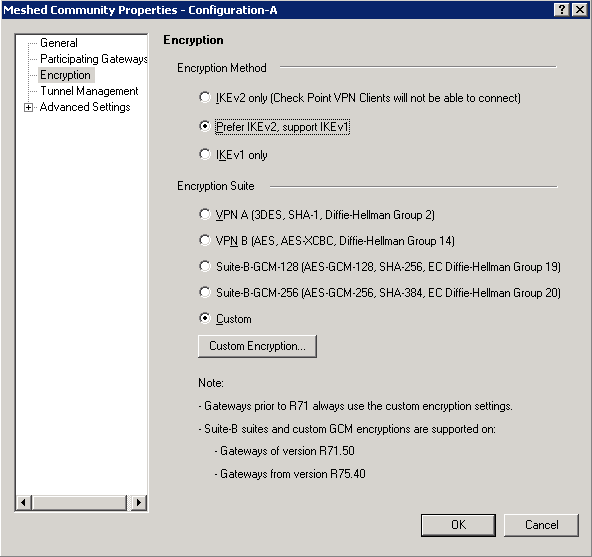
\includegraphics[width=0.592\textwidth]{img/checkpoint_1.png}
  \caption{VPN Community encryption properties}
  \label{fig:checkpoint_1}
\end{figure}

Either choose one of the encryption suites in the properties dialog
(figure \ref{fig:checkpoint_1}), or proceed to
``Custom Encryption...'', where you can set encryption and hash for
Phase 1 and 2 (figure \ref{fig:checkpoint_2}).

\begin{figure}[p]
  \centering
  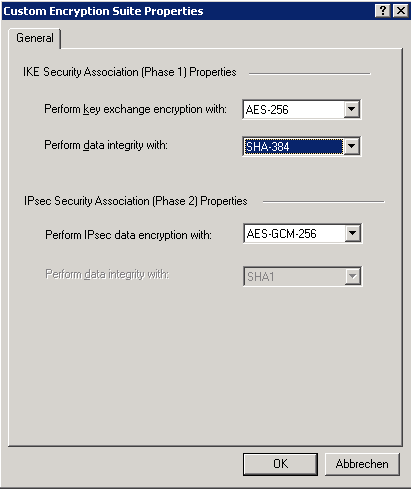
\includegraphics[width=0.411\textwidth]{img/checkpoint_2.png}
  \caption{Custom Encryption Suite Properties}
  \label{fig:checkpoint_2}
\end{figure}

The Diffie-Hellman groups and Perfect Forward Secrecy Settings can be
found under ``Advanced Settings'' / ``Advanced VPN Properties''
(figure \ref{fig:checkpoint_3}).

\begin{figure}[p]
  \centering
  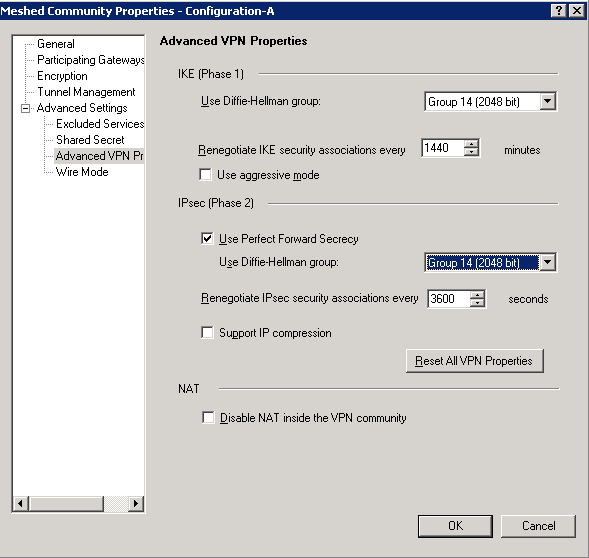
\includegraphics[width=0.589\textwidth]{img/checkpoint_3.png}
  \caption{Advanced VPN Properties}
  \label{fig:checkpoint_3}
\end{figure}


\subsubsection{Additional settings}
For remote Dynamic IP Gateways, the settings are not taken from the
community, but set in the ``Global Properties'' dialog under ``Remote
Access'' / ``VPN Authentication and Encryption''. Via the ``Edit...''
button, you can configure sets of algorithms that all gateways support
(figure \ref{fig:checkpoint_4}).

\begin{figure}[p]
  \centering
  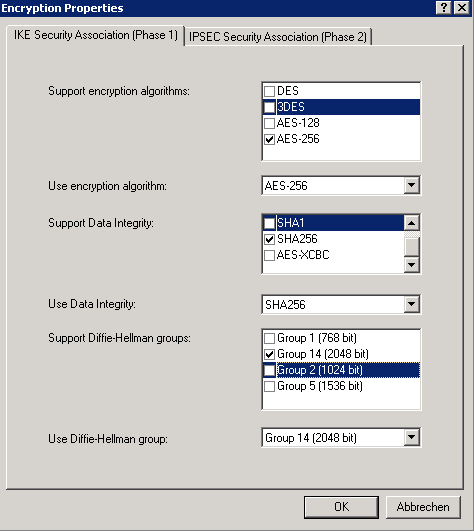
\includegraphics[width=0.474\textwidth]{img/checkpoint_4.png}
  \caption{Remote Access Encryption Properties}
  \label{fig:checkpoint_4}
\end{figure}

Please note that these settings restrict the available algorithms for
\textbf{all} gateways, and also influence the VPN client connections.

%\subsubsection{Justification for special settings (if needed)}

%\subsubsection{Limitations}

\subsubsection{References}
\begin{itemize*}
  \item Check Point \href{https://sc1.checkpoint.com/documents/R77/CP_R77_VPN_AdminGuide/html_frameset.htm}{VPN R77 Administration Guide} (may require a UserCenter account to access)
\end{itemize*}

%\subsubsection{How to test}

%% cipherstrings current 2013-12-09
% ---------------------------------------------------------------------- 
\FloatBarrier % the preceding section has several figures. Floating them too far away might get confusing for readers.

\subsection{OpenVPN}

\subsubsection{Tested with Versions}
\begin{itemize*}
  \item OpenVPN 2.3.10 from Ubuntu Xenial 16.04.1 LTS linked against openssl (libssl.so.1.0.0)
  \item OpenVPN 2.3.2 from Debian ``wheezy-backports'' linked against openssl (libssl.so.1.0.0)
  \item OpenVPN 2.2.1 from Debian Wheezy linked against openssl (libssl.so.1.0.0)
  \item OpenVPN 2.3.2 for Windows
\end{itemize*}

\subsubsection{Settings}

\paragraph{General}
We describe a configuration with certificate-based authentication; see
below for details on the \verb|easyrsa| tool to help you with that.

OpenVPN uses TLS only for authentication and key exchange. The
bulk traffic is then encrypted and authenticated with the OpenVPN
protocol using those keys.

Note that while the \verb|tls-cipher| option takes a list of ciphers
that is then negotiated as usual with TLS, the \verb|cipher|
and \verb|auth| options both take a single argument that must match on
client and server.

OpenVPN duplexes the tunnel into a data and a control channel. The control
channel is a usual TLS connection, the data channel currently uses 
encrypt-then-mac CBC, see \url{https://github.com/BetterCrypto/Applied-Crypto-Hardening/pull/91#issuecomment-75365286}


\paragraph{Server Configuration}
~\\
% the cipherlist here is config B without the ECDHE strings, because
% it must fit in 256 bytes...
% DO NOT CHANGE TO THE CIPHERSTRING MACRO!
\configfile{server.conf}{248-250}{Cipher configuration for OpenVPN (Server)}

\paragraph{Client Configuration}
Client and server have to use compatible configurations, otherwise they can't communicate.
The \verb|cipher| and \verb|auth| directives have to be identical.

% the cipherlist here is config B without the ECDHE strings, because
% it must fit in 256 bytes...
% DO NOT CHANGE TO THE CIPHERSTRING MACRO!
\configfile{client.conf}{44-45,115-121}{Cipher and TLS configuration for OpenVPN (Server)}

\subsubsection{Justification for special settings}
OpenVPN 2.3.1 changed the values that the \verb|tls-cipher| option
expects from OpenSSL to IANA cipher names. That means from that
version on you will get ``Deprecated TLS cipher name'' warnings for
the configurations above. You cannot use the selection strings from
section \ref{section:recommendedciphers} directly from 2.3.1 on, which
is why we give an explicit cipher list here.

In addition, there is a 256 character limit on configuration file line
lengths; that limits the size of cipher suites, so we dropped all
ECDHE suites and most CAMELLIA variants.

If maximal compatibility is required (and warnings are acceptable) the following
cipher list might be considered.

\begin{lstlisting}
tls-cipher DHE-RSA-AES256-GCM-SHA384:DHE-RSA-AES256-SHA256:DHE-RSA-AES128-GCM-SHA256:DHE-RSA-AES128-SHA256:DHE-RSA-CAMELLIA256-SHA:DHE-RSA-AES256-SHA:DHE-RSA-CAMELLIA128-SHA:DHE-RSA-AES128-SHA:CAMELLIA256-SHA:AES256-SHA:CAMELLIA128-SHA:AES128-SHA
\end{lstlisting}

The configuration shown above is compatible with all tested versions.


\subsubsection{References}
\begin{itemize*}
  \item OpenVPN Documentation: \emph{Security Overview} \url{https://openvpn.net/index.php/open-source/documentation/security-overview.html}
\end{itemize*}

%\subsubsection{How to test}


\subsubsection{Additional settings}

\paragraph{Key renegotiation interval}
The default for renegotiation of encryption keys is one hour
(\verb|reneg-sec 3600|). If you
transfer huge amounts of data over your tunnel, you might consider
configuring a shorter interval, or switch to a byte- or packet-based
interval (\verb|reneg-bytes| or \verb|reneg-pkts|).

\paragraph{Insecure ciphers}

Sweet32\footnote{\url{https://sweet32.info/}} is an attack on 64-bit block
ciphers, such as \verb|3DES| and \verb|Blowfish| in OpenVPN. The following
ciphers are affected, and should no longer be used:
\begin{itemize*}
  \item BF-*
  \item DES* (including 3DES variants)
  \item RC2-*
\end{itemize*}
The following ciphers are not affected:
\begin{itemize*}
  \item AES-*
  \item CAMELLIA-*
  \item SEED-*
\end{itemize*}
According to mitigation section on Sweet32 website\footnote{\url{https://sweet32.info/\#impact}}
users users should change the cipher from the DES or Blowfish to AES
(\verb|cipher AES-128-CBC|). If cipher change is not possible users can
mitigate the attack by forcing frequent rekeying (\verb|reneg-bytes 64000000|).

\paragraph{Fixing ``easy-rsa''}
When installing an OpenVPN server instance, you are probably using
\emph{easy-rsa} to generate keys and certificates.
The file \verb|vars| in the easyrsa installation directory has a
number of settings that should be changed to secure values:

\configfile{vars}{53-53,56-56,59-59}{Sane default values for OpenVPN (easy-rsa)}


This will enhance the security of the key generation by using RSA keys
with a length of 4096 bits, and set a lifetime of one year for the
server/client certificates and five years for the CA certificate. \textbf{NOTE: 4096 bits is only an example of how to do this with easy-rsa.} See also section \ref{section:keylengths} for a discussion on keylengths.

In addition, edit the \verb|pkitool| script and replace all occurrences
of \verb|sha1| with \verb|sha256|, to sign the certificates with
SHA256.

\subsubsection{Limitations}
Note that the ciphersuites shown by \verb|openvpn --show-tls| are \emph{known}, but not necessarily \emph{supported} \footnote{\url{https://community.openvpn.net/openvpn/ticket/304}}.

Which cipher suite is actually used can be seen in the logs:

\verb|Control Channel: TLSv1, cipher TLSv1/SSLv3 DHE-RSA-CAMELLIA256-SHA, 2048 bit RSA|


% ---------------------------------------------------------------------- 
\subsection{PPTP}

PPTP is considered insecure, Microsoft recommends to ``use a more secure VPN
tunnel''\footnote{\url{http://technet.microsoft.com/en-us/security/advisory/2743314}}.

There is a cloud service that cracks the underlying MS-CHAPv2
authentication protocol for the price of USD~200\footnote{\url{https://www.cloudcracker.com/blog/2012/07/29/cracking-ms-chap-v2/}},
and given the resulting MD4 hash, all PPTP traffic for a user can
be decrypted.

% ---------------------------------------------------------------------- 
\subsection{Cisco ASA}
The following settings reflect our recommendations as best as possible on the Cisco ASA platform. These are - of course - just settings regarding SSL/TLS (i.e. Cisco AnyConnect) and IPsec. For further security settings regarding this platform the appropriate Cisco guides should be followed.


\subsubsection{Tested with Versions}
\begin{itemize*}
  \item 9.1(3) - X-series model
\end{itemize*}

\subsubsection{Settings}
\begin{lstlisting}
crypto ipsec ikev2 ipsec-proposal AES-Fallback
 protocol esp encryption aes-256 aes-192 aes
 protocol esp integrity sha-512 sha-384 sha-256
crypto ipsec ikev2 ipsec-proposal AES-GCM-Fallback
 protocol esp encryption aes-gcm-256 aes-gcm-192 aes-gcm
 protocol esp integrity sha-512 sha-384 sha-256
crypto ipsec ikev2 ipsec-proposal AES128-GCM
 protocol esp encryption aes-gcm
 protocol esp integrity sha-512
crypto ipsec ikev2 ipsec-proposal AES192-GCM
 protocol esp encryption aes-gcm-192
 protocol esp integrity sha-512
crypto ipsec ikev2 ipsec-proposal AES256-GCM
 protocol esp encryption aes-gcm-256
 protocol esp integrity sha-512
crypto ipsec ikev2 ipsec-proposal AES
 protocol esp encryption aes
 protocol esp integrity sha-1 md5
crypto ipsec ikev2 ipsec-proposal AES192
 protocol esp encryption aes-192
 protocol esp integrity sha-1 md5
crypto ipsec ikev2 ipsec-proposal AES256
 protocol esp encryption aes-256
 protocol esp integrity sha-1 md5
crypto ipsec ikev2 sa-strength-enforcement
crypto ipsec security-association pmtu-aging infinite
crypto dynamic-map SYSTEM_DEFAULT_CRYPTO_MAP 65535 set pfs group14
crypto dynamic-map SYSTEM_DEFAULT_CRYPTO_MAP 65535 set ikev2 ipsec-proposal AES256-GCM AES192-GCM AES128-GCM AES-GCM-Fallback AES-Fallback
crypto map Outside-DMZ_map 65535 ipsec-isakmp dynamic SYSTEM_DEFAULT_CRYPTO_MAP
crypto map Outside-DMZ_map interface Outside-DMZ

crypto ikev2 policy 1
 encryption aes-gcm-256
 integrity null
 group 14
 prf sha512 sha384 sha256 sha
 lifetime seconds 86400
crypto ikev2 policy 2
 encryption aes-gcm-256 aes-gcm-192 aes-gcm
 integrity null
 group 14
 prf sha512 sha384 sha256 sha
 lifetime seconds 86400
crypto ikev2 policy 3
 encryption aes-256 aes-192 aes
 integrity sha512 sha384 sha256
 group 14
 prf sha512 sha384 sha256 sha
 lifetime seconds 86400
crypto ikev2 policy 4
 encryption aes-256 aes-192 aes
 integrity sha512 sha384 sha256 sha
 group 14
 prf sha512 sha384 sha256 sha
 lifetime seconds 86400
crypto ikev2 enable Outside-DMZ client-services port 443
crypto ikev2 remote-access trustpoint ASDM_TrustPoint0

ssl server-version tlsv1-only
ssl client-version tlsv1-only
ssl encryption dhe-aes256-sha1 dhe-aes128-sha1 aes256-sha1 aes128-sha1
ssl trust-point ASDM_TrustPoint0 Outside-DMZ
\end{lstlisting}

\subsubsection{Justification for special settings}
New IPsec policies have been defined which do not make use of ciphers that may be cause for concern. Policies have a "Fallback" option to support legacy devices.

3DES has been completely disabled as such Windows XP AnyConnect Clients will no longer be able to connect.

The Cisco ASA platform does not currently support RSA Keys above 2048bits.

Legacy ASA models (e.g. 5505, 5510, 5520, 5540, 5550) do not offer the possibility to configure for SHA256/SHA384/SHA512 nor AES-GCM for IKEv2 proposals.

\subsubsection{References}
\begin{itemize*}
  \item \url{http://www.cisco.com/en/US/docs/security/asa/roadmap/asaroadmap.html}
  \item \url{http://www.cisco.com/web/about/security/intelligence/nextgen_crypto.html}
\end{itemize*}

% add any further references or best practice documents here

%%\subsubsection{How to test}
% describe here or point the admin to tools (can be a simple footnote or \ref{} to  the tools section) which help the admin to test his settings.


% ---------------------------------------------------------------------- 
\subsection{Openswan}


\subsubsection{Tested with Version}
\begin{itemize*}
  \item Openswan 2.6.39 (Gentoo)
\end{itemize*}

\subsubsection{Settings}
Note: the available algorithms depend on your kernel configuration (when using protostack=netkey) and/or build-time options.

To list the supported algorithms
\begin{lstlisting}
$ ipsec auto --status | less
\end{lstlisting}
and look for 'algorithm ESP/IKE' at the beginning.

\begin{lstlisting}
aggrmode=no
# ike format: cipher-hash;dhgroup
# recommended ciphers:
# - aes
# recommended hashes:
# - sha2_256 with at least 43 byte PSK
# - sha2_512 with at least 86 byte PSK
# recommended dhgroups:
# - modp2048 = DH14
# - modp3072 = DH15
# - modp4096 = DH16
# - modp6144 = DH17
# - modp8192 = DH18
ike=aes-sha2_256;modp2048
type=tunnel
phase2=esp
# esp format: cipher-hash;dhgroup
# recommended ciphers configuration A:
# - aes_gcm_c-256 = AES_GCM_16
# - aes_ctr-256
# - aes_ccm_c-256 = AES_CCM_16
# - aes-256 
# additional ciphers configuration B:
# - camellia-256
# - aes-128
# - camellia-128
# recommended hashes configuration A:
# - sha2-256
# - sha2-384
# - sha2-512
# - null (only with GCM/CCM ciphers)
# additional hashes configuration B:
# - sha1
# recommended dhgroups: same as above
phase2alg=aes_gcm_c-256-sha2_256;modp2048
salifetime=8h
pfs=yes
auto=ignore
\end{lstlisting}

\subsubsection{How to test}
Start the vpn and using
\begin{lstlisting}
$ ipsec auto --status | less
\end{lstlisting}
and look for 'IKE algorithms wanted/found' and 'ESP algorithms wanted/loaded'.

\subsubsection{References}
%\todo{more specific References??}
\begin{itemize*}
  \item \url{https://www.openswan.org/}
\end{itemize*}


\subsection{tinc}
\subsubsection{Tested with Version}
\begin{itemize*}
  \item tinc 1.0.23 from Gentoo linked against OpenSSL 1.0.1e
  \item tinc 1.0.23 from Sabayon linked against OpenSSL 1.0.1e
\end{itemize*}

\paragraph*{Defaults}\mbox{}\\
tinc uses 2048 bit RSA keys, Blowfish-CBC, and SHA1 as default settings and suggests the usage of CBC mode ciphers.
Any key length up to 8192 is supported and it does not need to be a power of two. OpenSSL Ciphers and Digests are supported by tinc.

\paragraph*{Settings}\mbox{}\\
Generate keys with
\begin{lstlisting}[breaklines]
tincd -n NETNAME -K8192
\end{lstlisting}
Old keys will not be deleted (but disabled), you have to delete them manually. Add the following lines to your tinc.conf on all machines
\configfile{tinc.conf}{3-4}{Cipher and digest selection in tinc}

\paragraph*{References}\mbox{}\\
\begin{itemize}
\item tincd(8) man page
\item tinc.conf(5) man page
\item \href{http://www.tinc-vpn.org/pipermail/tinc/2014-January/003538.html}{tinc mailinglist: http://www.tinc-vpn.org/pipermail/tinc/2014-January/003538.html}
\end{itemize}


% ---------------------------------------------------------------------- 
%%\subsection{Juniper VPN}
%%\todo{write this subsubsection. AK: ask Hannes}




% ---------------------------------------------------------------------- 
%\subsection{L2TP over IPSec}
%\todo{write this subsubsection}




% ---------------------------------------------------------------------- 
%\subsection{Racoon}
%\todo{write this subsubsection}



\section{PGP/GPG - Pretty Good Privacy}
\label{sec:pgpgpg-pretty-good}
% hack.
\gdef\currentsectionname{GPG}
\gdef\currentsubsectionname{GnuPG}

The OpenPGP protocol\footnote{\url{https://tools.ietf.org/search/rfc4880}} defines a set of asymmetric- and symmetric encryption algorithms, signature methods and compression protocols. GnuPG\footnote{\url{https://gnupg.org/}}, a FOSS implementation of the OpenPGP standard, is widely used for mail encryption.
 
GnuPG signs a message, encrypts it symmetrically and encrpts the symmetric key and the hash with Bob's public key asymmetrically.

Research on SHA-1 conducted back in 2005\footnote{\url{https://www.schneier.com/blog/archives/2005/02/sha1\_broken.html}} as well as the first practical successful collision in early 2017\footnote{\url{https://shattered.io/}} has made clear that collision attacks are a real threat to the security of the SHA-1 hash function. Since SHA-1 is defined as a must implementation by the OpenPGP specification, GnuPG is still using it. Currently settings should be adapted to preferably avoid using SHA-1. 

When using GnuPG, there are a couple of things to take care of:
\begin{itemize*}
  \item keylengths (see section \ref{section:keylengths})
  \item randomness (see section \ref{section:RNGs})
  \item preference of symmetric encryption algorithm (see section \ref{section:CipherSuites})
  \item preference of hash function (see section \ref{section:CipherSuites})
\end{itemize*}

Properly dealing with key material, passphrases and the web-of-trust is outside of the scope of this document. The GnuPG
website\footnote{\url{http://www.gnupg.org}} has a good tutorial on GnuPG.

After 31 December 2017 GnuPG version 2.0.x is no longer supported and shall not be used
anymore\footnote{\url{https://lists.gnupg.org/pipermail/gnupg-announce/2017q3/000413.html}}. Use the new long term
version 2.1 instead.

\subsubsection{Hashing}
Avoid SHA-1 by preferring better hashing methods. GnuPG. Edit \$HOME/.gnupg/gpg.conf:

\configfile{gpg.conf}{208-210}{Digest selection in GnuPG}

\subsection{Key Generation}
\gdef\currentsectionname{GPG}
\gdef\currentsubsectionname{GnuPG}
Because of lack of forward secrecy \ref{subsection:PFS} in OpenPGP it is preferable to use large asymmetric keys for long term
communication protection. A RSA key of 4096 bits should provide enough confidentiality for the next 10 years\footnote{\url{https://www.keylength.com}}.

\configfile{new-key-generation.txt}{}{New key generation with GnuPG version 2.1}

\configfile{params.txt}{}{Parameters for key generation with GnuPG version 2.1}

The preferences parameters S9 to Z1 correspond to AES256, CAMELLIA256, AES192, CAMELLIA192, AES, CAMELLIA128, TWOFISH,
SHA512, SHA384, SHA256, BZIP2, ZLIB and ZIP. The parameters 3DES, SHA-1 and uncompressed are set automatically by GnuPG.

\subsection{ECC - Elliptic Curve Cryptography}
Since the release of GnuPG version 2.1 end-2014\footnote{\url{https://www.gnupg.org/faq/whats-new-in-2.1.html}} ECC is supported. Older versions though are still widely used therefore ECC is not yet applicable in practice. 

%\subsubsection{PGP / GPG Operations}

%% Ciphering - Unciphering operations
%%% TOO COMPLEX. Make a pointer to a good GPG tutorial

%% Signing / checking signatures
%%% TOO COMPLEX. Make a pointer to a good GPG tutorial

%\subsubsection{Trusted Keys}

%%Explain that a key by himself is not trustable.  Chain of trust principle.

%%% TOO COMPLEX. Make a pointer to a good GPG tutorial

%\subsection{Available implementations and mails plugins}

%% Microsoft Windows (Symantec for Outlook? GnuPG + ....)
%%% TOO COMPLEX. Make a pointer to a good GPG tutorial

%% Linux (GnuPG + Enigmail for Thunderbird)

%%% TOO COMPLEX. Make a pointer to a good GPG tutorial
%% Mac OS X (GnuPG + GPGMail)
%%% TOO COMPLEX. Make a pointer to a good GPG tutorial



%\section{seclayer-tcp}
%\input{practical_settings/seclayer_tcp}
\section{IPMI, ILO and other lights out management solutions}
\label{sec:ipmi-ilo-other}
\input{practical_settings/ipmi}
%%\section{SIP}
%%\todo{AK: ask Klaus. Write this section, Klaus??? }
\section{Instant Messaging Systems}
\label{sec:inst-mess-syst}
%%---------------------------------------------------------------------- 
\subsection{General server configuration recommendations}

For servers, we mostly recommend to apply what's proposed by the \emph{Peter's manifesto}\footnote{\url{https://github.com/stpeter/manifesto}}.

In short:
\begin{itemize*}
    \item require the use of TLS for both client-to-server and server-to-server connections
    \item prefer or require TLS cipher suites that enable forward secrecy
    \item deploy certificates issued by well-known and widely-deployed certification authorities (CAs)
\end{itemize*}

The last point being out-of-scope for this section, we will only cover the first two points.

\subsection{ejabberd}

\subsubsection{Tested with Versions}
\begin{itemize*}
  \item Debian Wheezy 2.1.10-4+deb7u1
\end{itemize*}

\subsubsection{Settings}
ejabberd is one of the popular Jabber server. In order to be compliant
with the manifesto, you should adapt your configuration\footnote{\url{http://www.process-one.net/docs/ejabberd/guide_en.html}}:
\begin{lstlisting}
{listen,
 [
  {5222, ejabberd_c2s, [
                        {access, c2s},
                        {shaper, c2s_shaper},
                        {max_stanza_size, 65536},
                        starttls,
                        starttls_required, 
                        {certfile, "/etc/ejabberd/ejabberd.pem"}
                       ]},
  {5269, ejabberd_s2s_in, [
                           {shaper, s2s_shaper},
                           {max_stanza_size, 131072}
                          ]},

  %%% Other input ports
]}.
{s2s_use_starttls, required_trusted}.
{s2s_certfile, "/etc/ejabberd/ejabberd.pem"}.
\end{lstlisting}

\subsubsection{Additional settings}
Older Versions of ejabberd ($ < $ 2.0.0) need to be patched\footnote{\url{http://hyperstruct.net/2007/06/20/installing-the-startcom-ssl-certificate-in-ejabberd/}} to be able to parse all of the certificates in the CA chain.

Newer versions of ejabberd now support specifying the cipher string in the config file. See the commit message: \url{https://github.com/processone/ejabberd/commit/1dd94ac0d06822daa8c394ea2da20d91c8209124}. However, this change did not yet make it into the stable release at the time of this writing. 


\subsubsection{References}


\subsubsection{How to test}
\begin{itemize*}
  \item \url{https://xmpp.net} is a practical website to test Jabber server configurations.
\end{itemize*}


%%---------------------------------------------------------------------- 
\subsection{Chat privacy - Off-the-Record Messaging (OTR)}

The OTR protocol works on top of the Jabber protocol\footnote{\url{https://otr.cypherpunks.ca/Protocol-v3-4.0.0.html}}.  
It adds to popular chat clients (Adium, Pidgin...) the following properties for encrypted chats:
\begin{itemize*}
  \item Authentication
  \item Integrity
  \item Confidentiality
  \item Forward secrecy
\end{itemize*}

It basically uses Diffie-Hellman, AES and SHA1. Communicating over an insecure instant messaging network, OTR can be used for end to end encryption.

There are no specific configurations required but the protocol itself is worth to be mentioned.


%%---------------------------------------------------------------------- 
\subsection{Charybdis}
There are numerous implementations of IRC servers.  In this section, we choose \emph{Charybdis} which serves as basis for \emph{ircd-seven}\footnote{\url{https://dev.freenode.net/redmine/projects/ircd-seven}}, developed and used by freenode. Freenode is actually the biggest IRC network\footnote{\url{http://irc.netsplit.de/networks/top10.php}}. \emph{Charybdis} is part of the \emph{Debian} \& \emph{Ubuntu} distributions.

\begin{lstlisting}
/* Extensions */
# Some modules 
#loadmodule "extensions/chm_sslonly_compat.so";
loadmodule "extensions/extb_ssl.so";
# Some other modules

serverinfo {
  /* Standard piece of information */
  
  ssl_private_key = "etc/test.key";
  ssl_cert = "etc/test.cert";
  ssl_dh_params = "etc/dh.pem";
  # set ssld_count as number of cores - 1
  ssld_count = 1; 
};

listen {
  /* Standard ports */
  sslport = 6697;

  /* IPv6 configuration */
};
\end{lstlisting}


%%---------------------------------------------------------------------- 
\subsection{SILC}

SILC\footnote{\url{http://www.silcnet.org/} and
\url{https://en.wikipedia.org/wiki/SILC_(protocol)}} is instant messaging
protocol publicly released in 2000. SILC is a per-default secure chat protocol
thanks to a generalized usage of symmetric encryption. Keys are generated by
the server meaning that if compromised, communication could be compromised.

The protocol is not really popular anymore.


\section{Database Systems}
\label{sec:database-systems}
%%\subsection{Database Systems}
% This list is based on : http://en.wikipedia.org/wiki/Relational_database_management_system#Market_share

%% ---------------------------------------------------------------------- 
\subsection{Oracle}
\subsubsection{Tested with Versions}
\todo{not tested yet}


\subsubsection{References}
\begin{itemize*}
  \item Technical safety requirements by \emph{Deutsche Telekom AG} (German). Please read section 17.12 or pages 129 and following (Req 396 and Req 397) about SSL and ciphersuites \url{http://www.telekom.com/static/-/155996/7/technische-sicherheitsanforderungen-si}
\end{itemize*}



%% ---------------------------------------------------------------------- 
%%\subsection{SQL Server}
%%\todo{write this}



%% ---------------------------------------------------------------------- 
\subsection{MySQL}


\subsubsection{Tested with Versions}
\begin{itemize*}
  \item Debian Wheezy and MySQL 5.5
\end{itemize*}


\subsubsection{Settings}
\paragraph*{my.cnf}
\begin{lstlisting}
[mysqld]
ssl
ssl-ca=/etc/mysql/ssl/ca-cert.pem
ssl-cert=/etc/mysql/ssl/server-cert.pem
ssl-key=/etc/mysql/ssl/server-key.pem
ssl-cipher=%*\cipherStringB*)
\end{lstlisting}


%\subsubsection{Additional settings}


%\subsubsection{Justification for special settings (if needed)}
% in case you have the need for further justifications why you chose this and that setting or if the settings do not fit into the standard Variant A or Variant B schema, please document this here


\subsubsection{References}
\begin{itemize*}
  \item MySQL Documentation on SSl Connections: \url{https://dev.mysql.com/doc/refman/5.5/en/ssl-connections.html}
\end{itemize*}


\subsubsection{How to test}
After restarting the server run the following query to see if the ssl settings are correct:
\begin{lstlisting}
show variables like '%ssl%';
\end{lstlisting}


%% ---------------------------------------------------------------------- 
\subsection{DB2}
\subsubsection{Tested with Version}
\todo{not tested}


\subsubsection{Settings}
\paragraph{ssl\_cipherspecs:}
In the link above the whole SSL-configuration is described in-depth. The following command shows only how to set the recommended ciphersuites.
\begin{lstlisting}
# recommended and supported ciphersuites 

db2 update dbm cfg using SSL_CIPHERSPECS 
TLS_RSA_WITH_AES_256_CBC_SHA256,
TLS_RSA_WITH_AES_128_GCM_SHA256,
TLS_RSA_WITH_AES_128_CBC_SHA256,
TLS_ECDHE_RSA_WITH_AES_128_GCM_SHA256,
TLS_ECDHE_ECDSA_WITH_AES_128_GCM_SHA256,
TLS_ECDHE_RSA_WITH_AES_128_CBC_SHA256,
TLS_ECDHE_ECDSA_WITH_AES_128_CBC_SHA256,
TLS_RSA_WITH_AES_256_GCM_SHA384,
TLS_ECDHE_RSA_WITH_AES_256_GCM_SHA384,
TLS_ECDHE_ECDSA_WITH_AES_256_GCM_SHA384,
TLS_ECDHE_RSA_WITH_AES_256_CBC_SHA384,
TLS_ECDHE_ECDSA_WITH_AES_256_CBC_SHA384,
TLS_ECDHE_RSA_WITH_AES_256_CBC_SHA,
TLS_ECDHE_ECDSA_WITH_AES_256_CBC_SHA,
TLS_RSA_WITH_AES_256_CBC_SHA,
TLS_RSA_WITH_AES_128_CBC_SHA,
TLS_ECDHE_RSA_WITH_AES_128_CBC_SHA,
TLS_ECDHE_ECDSA_WITH_AES_128_CBC_SHA
\end{lstlisting}


\subsubsection{References}
\begin{itemize*}
  \item IMB Db2 Documentation on \emph{Supported cipher suites} \url{http://pic.dhe.ibm.com/infocenter/db2luw/v9r7/index.jsp?topic=\%2Fcom.ibm.db2.luw.admin.sec.doc\%2Fdoc\%2Fc0053544.html}
\end{itemize*}

%% ---------------------------------------------------------------------- 

\subsection{PostgreSQL}
\subsubsection{Tested with Versions}
\begin{itemize*}
  \item Debian Wheezy and PostgreSQL 9.1
  \item Linux Mint 14 nadia / Ubuntu 12.10 quantal with PostgreSQL 9.1+136 and OpenSSL 1.0.1c
\end{itemize*}


\subsubsection{Settings}
To start in SSL mode the server.crt and server.key must exist in the server's data directory \$PGDATA.

Starting with version 9.2, you have the possibility to set the path manually.

\begin{lstlisting}
ssl_key_file = '/your/path/server.key'
ssl_cert_file = '/your/path/server.crt'
ssl_ca_file = '/your/path/root.crt'
\end{lstlisting}

\paragraph*{postgresql.conf}
\begin{lstlisting}
#>=8.3
ssl = on 
ssl_ciphers = '%*\cipherStringB*)'
\end{lstlisting}


\subsubsection{References}
\begin{itemize*}
  \item It's recommended to read \url{http://www.postgresql.org/docs/9.1/interactive/runtime-config-connection.html\#RUNTIME-CONFIG-CONNECTION-SECURITY} (please edit the version with your preferred one).
  \item PostgreSQL Documentation on \emph{Secure TCP/IP Connections with SSL}: \url{http://www.postgresql.org/docs/9.1/static/ssl-tcp.html}
  \item PostgreSQL Documentation on \emph{host-based authentication}: \url{http://www.postgresql.org/docs/current/static/auth-pg-hba-conf.html}
\end{itemize*}


\subsubsection{How to test}
To test your ssl settings, run psql with the sslmode parameter:
\begin{lstlisting}
psql "sslmode=require host=postgres-server dbname=database" your-username
\end{lstlisting}


\section{Intercepting proxy solutions and reverse proxies}
\label{sec:interc-proxy-solut}
%hack.
\gdef\currentsectionname{Proxies}
%%\subsection{Intercepting proxy solutions and reverse proxies}

Within enterprise networks and corporations with increased levels of paranoia or at least some defined security requirements it is common \textbf{not} to allow direct connections to the public internet.

For this reason proxy solutions are deployed on corporate networks to intercept and scan the traffic for potential threats within sessions.

For encrypted traffic there are four options:

\begin{itemize*}
  \item Block the connection because it cannot be scanned for threats.
  \item Bypass the threat-mitigation and pass the encrypted session to the client, which results in a situation where malicious content is transferred directly to the client without visibility to the security system.
  \item Intercept (i.e. terminate) the session at the proxy, scan there and re-encrypt the session towards the client (effectively MITM).
  \item Deploy special Certificate Authorities to enable Deep Packet Inspection on the wire.
\end{itemize*}

While the latest solution might be the most "up to date", it arises a new front in the context of this paper, because the most secure part of a client's connection could only be within the corporate network, if the proxy-server handles the connection to the destination server in an insecure manner.

Conclusion: Don't forget to check your proxy solutions SSL-capabilities. Also do so for your reverse proxies!

%% ---------------------------------------------------------------------- 
% who was the author of this section?
% can we have this either tested or removed?
%\subsection{Squid}
%As of squid-3.2.7 (01 Feb 2013) there is support for the OpenSSL NO\_Compression option within squid config (CRIME attack) and if you combine that in the config file, with an enforcement of the server cipher preferences (BEAST Attack) you are safe.
%
%
%\todo{UNTESTED!}
%\configfile{squid.conf}{1363-1363,1379-1379}{Cipher selection and SSL options in Squid}
%%% http://forum.pfsense.org/index.php?topic=63262.0
%%\todo{UNTESTED!}
%% see squid.conf, repeating the options here does not help.
%\todo{Patch here? Definitely working for 3.2.6!}
%For squid Versions before 3.2.7 use this patch against a vanilla source-tree:
%\begin{lstlisting}
%--- support.cc.ini      2013-01-09 02:41:51.000000000 +0100
%+++ support.cc  2013-01-21 16:13:32.549383848 +0100
%@@ -400,6 +400,11 @@
%         "NO_TLSv1_2", SSL_OP_NO_TLSv1_2
%     },
% #endif
%+#ifdef SSL_OP_NO_COMPRESSION
%+    {
%+        "NO_Compression", SSL_OP_NO_COMPRESSION
%+    },
%+#endif
%     {
%         "", 0
%     },
%\end{lstlisting}
%
%
%% ---------------------------------------------------------------------- 
\subsection{Bluecoat}
%% https://kb.bluecoat.com/index?page=content&id=KB5549
\subsubsection{Tested with Versions}
\begin{itemize*}
  \item SGOS 6.5.x
\end{itemize*}

BlueCoat Proxy SG Appliances can be used as forward and reverse proxies. The reverse proxy feature is rather under-developed, and while it is possible and supported, there only seems to be limited use of this feature "in the wild" - nonetheless there are a few cipher suites to choose from, when enabling SSL features.

\paragraph*{Only allow TLS 1.0,1.1 and 1.2 protocols:}
~
\begin{lstlisting}
$conf t
$(config)ssl
$(config ssl)edit ssl-device-profile default
$(config device-profile default)protocol tlsv1 tlsv1.1 tlsv1.2
  ok
\end{lstlisting}

\paragraph*{Select your accepted cipher-suites:}
~
\begin{lstlisting}
$conf t
Enter configuration commands, one per line.  End with CTRL-Z.
$(config)proxy-services
$(config proxy-services)edit ReverseProxyHighCipher
$(config ReverseProxyHighCipher)attribute cipher-suite
Cipher#  Use        Description        Strength
-------  ---  -----------------------  --------
      1  yes            AES128-SHA256      High
      2  yes            AES256-SHA256      High
      3  yes               AES128-SHA    Medium
      4  yes               AES256-SHA      High
      5  yes       DHE-RSA-AES128-SHA      High
      6  yes       DHE-RSA-AES256-SHA      High
               [...]
     13  yes          EXP-RC2-CBC-MD5    Export

Select cipher numbers to use, separated by commas: 2,5,6
  ok
\end{lstlisting}

The same protocols are available for forward proxy settings and should be adjusted accordingly:
In your local policy file add the following section:
\begin{lstlisting}
<ssl>
    DENY server.connection.negotiated_ssl_version=(SSLV2, SSLV3)
\end{lstlisting}

Disabling protocols and ciphers in a forward proxy environment could lead to unexpected results on certain (misconfigured?) webservers (i.e. ones accepting only SSLv2/3 protocol connections)


%% ---------------------------------------------------------------------- 
\subsection{HAProxy}
% See http://www.haproxy.org/
% See https://timtaubert.de/blog/2014/11/the-sad-state-of-server-side-tls-session-resumption-implementations/
% See http://cbonte.github.io/haproxy-dconv/configuration-1.5.html#5.1-npn
% See http://cbonte.github.io/haproxy-dconv/configuration-1.5.html#3.2-tune.ssl.cachesize
% See https://kura.io/2014/07/02/haproxy-ocsp-stapling/
% See https://kura.io/2015/01/27/hpkp-http-public-key-pinning-with-haproxy/

HAProxy can be used as loadbalancer and proxy for TCP and HTTP-based applications. Since version 1.5 it supports SSL and IPv6.

\subsubsection{Tested with Versions}
\begin{itemize*}
  \item HAProxy 1.5.11 with OpenSSL 1.0.1e on Debian Wheezy
\end{itemize*}

\subsubsection{Settings}
\configfile{haproxy.cfg}{1-4}{global configuration}
\configfile{haproxy.cfg}{21-25}{frontend configuration}
\configfile{haproxy.cfg}{27-33}{backend configuration}

\subsubsection{Additional Settings}
\paragraph*{Enable \ac{NPN} Support:}
~
\begin{lstlisting}
	bind *:443 ssl crt server.pem npn "http/1.1,http/1.0"
\end{lstlisting}
Append the npn command in the frontend configuration of HAProxy.

\paragraph*{Enable OCSP stapling:}
~
HAProxy supports since version 1.5.0 OCSP stapling. To enable it you have to generate the OCSP singing file in the same folder, with the same name as your certificate file plus the extension .ocsp. (e.g. your certificate file is named server.crt then the OCSP file have to be named server.crt.oscp)\\
To generate the OCSP file use these commands:
\begin{lstlisting}
openssl x509 -in your.certificate.crt -noout -ocsp_uri # <- get your ocsp uri
openssl ocsp -noverify -issuer ca.root.cert.crt -cert your.certificate.crt -url "YOUR OCSP URI" -respout your.certificate.crt.ocsp
\end{lstlisting}
Reload HAProxy and now OCSP stapling should be enabled.\\
Note: This OCSP signature file is only valid for a limited time. The simplest way of updating this file is by using cron.daily or something similar.

\paragraph*{Enable \ac{HPKP}:}
~
Get certificate informations:
\begin{lstlisting}
openssl x509 -in server.crt -pubkey -noout | openssl rsa -pubin -outform der | openssl dgst -sha256 -binary | base64
\end{lstlisting}
Then you append the returned string in the HAProxy configuration. Add the following line to the backend configuration:
\begin{lstlisting}
rspadd Public-Key-Pins:\ pin-sha256="YOUR_KEY";\ max-age=15768000;\ includeSubDomains
\end{lstlisting}
Reload HAProxy and HPKP should now be enabled.\\
Note: Keep in mind to generate a backup key in case of problems with your primary key file.

\subsubsection{How to test}
See appendix \ref{cha:tools}

%% ---------------------------------------------------------------------- 
\subsection{Pound}
% See http://www.apsis.ch/pound
% See https://help.ubuntu.com/community/Pound

\subsubsection{Tested with Versions}
\begin{itemize*}
  \item Pound 2.6
\end{itemize*}

\subsubsection{Settings}
\configfile{pound.cfg}{31}{HTTPS Listener in Pound}


%% ---------------------------------------------------------------------- 
\subsection{stunnel}
% See https://www.stunnel.org/

\subsubsection{Tested with Versions}
\begin{itemize*}
  \item stunnel 4.53-1.1ubuntu1 on Ubuntu 14.04 Trusty with OpenSSL 1.0.1f, without disabling Secure Client-Initiated Renegotiation
  \item stunnel 5.02-1 on Ubuntu 14.04 Trusty with OpenSSL 1.0.1f
  \item stunnel 4.53-1.1 on Debian Wheezy with OpenSSL 1.0.1e, without disabling Secure Client-Initiated Renegotiation
\end{itemize*}

\subsubsection{Settings}
\configfile{stunnel.conf}{48-55}{HTTPS Listener in Pound}

\subsubsection{Additional information}
Secure Client-Initiated Renegotiation can only be disabled for stunnel versions >= 4.54, when the renegotiation parameter has been added (See changelog).

\subsubsection{References} 
\begin{itemize*}
  \item stunnel documentation: \url{https://www.stunnel.org/static/stunnel.html}
  \item stunnel changelog: \url{https://www.stunnel.org/sdf_ChangeLog.html}
\end{itemize*}


\subsubsection{How to test} 
See appendix \ref{cha:tools}



%%% Local Variables: 
%%% mode: latex
%%% TeX-master: "applied-crypto-hardening"
%%% End: 

%%
\chapter{Theory}
%\epigraph{``Number theorists are like lotus-eaters - having tasted this food they can never give it up.''}{-- Leopold Kronecker}
\label{chapter:Theory}
\section{Overview}
\label{sec:TheoryOverview}


\epigraph{``The balance between freedom and security is a delicate one.''}{Mark Udall, american politician}

This chapter provides the necessary background information on why chapter \ref{chapter:PracticalSettings} recommended \textit{cipher string B}.

We start off by explaining the structure of cipher strings in section \ref{subsection:architecture} (architecture) and define \ac{PFS} in \ref{subsection:PFS}. Next we present \textit{Cipher String A} and \textit{Cipher String B} in section \ref{section:recommendedciphers}. This concludes the section on cipher strings. In theory, the reader should now be able to construct his or her own cipher string. However, the question why certain settings were chosen still remains. To answer this part, we need to look at recommended keylengths, problems in specific algorithms and hash functions and other cryptographic parameters. As mentioned initially in section \ref{section:relatedPublications}, the ENISA~\cite{ENISA2013}, ECRYPT 2~\cite{ii2011ecrypt} and BSI~\cite{TR02102} reports go much more into these topics and should be consulted in addition.

We try to answer the questions by explaining issues with random number generators (section \ref{section:RNGs}), keylengths (section \ref{section:keylengths}), current issues in ECC (section \ref{section:EllipticCurveCryptography}), a note of warning on SHA-1 (section \ref{section:SHA}) and some comments on Diffie Hellman key exchanges (section \ref{section:DH}). All of this is important in understanding why certain choices were made for \textit{Cipher String A and B}. However, for most system administrators, the question of compatibility is one of the most pressing ones.  Having the freedom to be compatible with any client (even running on outdated operating systems) of course, reduces the security of our cipher strings. We address these topics in section \ref{subsection:compatibility}. All these sections will allow a system administrator to balance his or her needs for strong encryption with usability and compatibility.

Last but not least, we finish this chapter by talking about issues in PKIs (section \ref{section:PKIs}), Certificate Authorities and on hardening a PKI.  Note that these last few topics deserve a book on their own. Hence this guide can only mention a few current topics in this area.

%%% Local Variables: 
%%% mode: latex
%%% TeX-master: "../applied-crypto-hardening"
%%% End: 

\section{Cipher suites}
\label{section:CipherSuites}
\todo{team: section \ref{section:CipherSuites} is currently a bit messy. Re-do it}


\subsection{Architectural overview }
\label{subsection:architecture}
%%\subsection{Architectural overview }

This section defines some terms which will be used throughout this guide.


A cipher suite is a standardized collection of key exchange algorithms, encryption 
algorithms (ciphers) and Message authentication codes (MAC) algorithm that provides
authenticated encryption schemes. It consists of the following components:

\begin{description}

  \item[Key exchange protocol:]
``An (interactive) key exchange protocol is a method whereby parties who do not 
share any secret information can generate a shared, secret key by communicating 
over a public channel. The main property guaranteed here is that an 
eavesdropping adversary who sees all the messages sent over the communication 
line does not learn anything about the resulting secret key.''~\cite{katz2008introduction}

Example: \texttt{DHE}

  \item[Authentication:]
The client authenticates the server by its certificate. Optionally the server 
may authenticate the client certificate.

Example: \texttt{RSA}

  \item[Cipher:]
The cipher is used to encrypt the message stream. It also contains the key size
and mode used by the suite.

Example: \texttt{AES256}

  \item[Message authentication code (MAC):]
A MAC ensures that the message has not been tampered with (integrity).

Examples: \texttt{SHA256}

  \item[Authenticated Encryption with Associated Data (AEAD):]
AEAD is a class of authenticated encryption block-cipher modes
which take care of encryption as well as authentication (e.g. GCM, CCM mode). 

Example: \texttt{AES256-GCM}



\begin{figure}[h]
\makebox[\textwidth]{
\framebox[1.1\width]{ \texttt{DHE} }--\framebox[1.1\width]{ \texttt{RSA} }--\framebox[1.1\width]{ \texttt{AES256} }--\framebox[1.1\width]{ \texttt{SHA256} } }
\caption{Composition of a typical cipher string}
\end{figure}
\end{description}
%
\paragraph*{A note on nomenclature:} there are two common naming schemes for cipher strings -- IANA names (see appendix \ref{cha:links}) and the more well known OpenSSL names. In this document we will always use OpenSSL names unless a specific service uses IANA names.



\subsection{Forward Secrecy}
\label{subsection:PFS}
%%\subsection{Forward Secrecy}
Forward Secrecy or Perfect Forward Secrecy is a property of a cipher suite 
that ensures confidentiality even if the server key has been compromised.
Thus if traffic has been recorded it can not be decrypted even if an adversary
has got hold of the server key
\footnote{\url{https://en.wikipedia.org/wiki/Forward\_secrecy}}
\footnote{\url{https://www.eff.org/deeplinks/2013/08/pushing-perfect-forward-secrecy-important-web-privacy-protection}}
\footnote{\url{http://news.netcraft.com/archives/2013/06/25/ssl-intercepted-today-decrypted-tomorrow.html}}.



\subsection{Recommended cipher suites}
\label{section:recommendedciphers}
%%\subsection{Recommended cipher suites}

In principle system administrators who want to improve their communication security
have to make a difficult decision between effectively locking out some users and
keeping high cipher suite security while supporting as many users as possible.
The website \url{https://www.ssllabs.com/} gives administrators and security engineers
a tool to test their setup and compare compatibility with clients. The authors made
use of ssllabs.com to arrive at a set of cipher suites which we will recommend
throughout this document.

%\textbf{Caution: these settings can only represent a subjective
%choice of the authors at the time of writing. It might be a wise choice to
%select your own and review cipher suites based on the instructions in section
%\ref{section:ChoosingYourOwnCipherSuites}}.


\subsubsection{Configuration A: Strong ciphers, fewer clients}

At the time of writing, our recommendation is to use the following set of strong cipher
suites which may be useful in an environment where one does not depend on many,
different clients and where compatibility is not a big issue.  An example
of such an environment might be machine-to-machine communication or corporate
deployments where software that is to be used can be defined without restrictions.


We arrived at this set of cipher suites by selecting:

\begin{itemize*}
  \item TLS 1.2
  \item Perfect forward secrecy / ephemeral Diffie Hellman
  \item strong MACs (SHA-2) or
  \item GCM as Authenticated Encryption scheme
\end{itemize*}

This results in the OpenSSL string:
\ttbox{EDH+aRSA+AES256:EECDH+aRSA+AES256:!SSLv3'}

%$\implies$ resolves to 
%
%\begin{verbatim}
%openssl ciphers -V $string
%\end{verbatim}



%\todo{make a column for cipher chaining mode} --> not really important, is it?
\ctable[caption={Configuration A ciphers},label=tab:conf-a]{lllllll}{}{%
\FL \textbf{ID}   & \textbf{OpenSSL Name}       & \textbf{Version} & \textbf{KeyEx} & \textbf{Auth} & \textbf{Cipher} & \textbf{MAC}
\ML \texttt{0x009F} & DHE-RSA-AES256-GCM-SHA384   & TLSv1.2          & DH             &  RSA          & AESGCM(256)     & AEAD
\NN \texttt{0x006B} & DHE-RSA-AES256-SHA256       & TLSv1.2          & DH             &  RSA          & AES(256) (CBC)  & SHA256
\NN \texttt{0xC030} & ECDHE-RSA-AES256-GCM-SHA384 & TLSv1.2          & ECDH           &  RSA          & AESGCM(256)     & AEAD
\NN \texttt{0xC028} & ECDHE-RSA-AES256-SHA384     & TLSv1.2          & ECDH           &  RSA          & AES(256) (CBC)  & SHA384
\LL}

\paragraph*{Compatibility:}

At the time of this writing only Win 7 and Win 8.1 crypto stack,
OpenSSL $\ge$ 1.0.1e, Safari 6 / iOS 6.0.1 and Safari 7 / OS X 10.9
are covered by that cipher string.

% XXX author: (Adi) this depends on the chosing your own cipher chapter XXX
%In case you need to support other/different clients, see information
%about choosing your own cipher string in section
%\ref{section:ChoosingYourOwnCipherSuites}.

\subsubsection{Configuration B: Weaker ciphers but better compatibility}

In this section we propose a slightly weaker set of cipher suites.  For
example, there are known weaknesses for the SHA-1 hash function that is
included in this set.  The advantage of this set of cipher suites is not only
better compatibility with a broad range of clients, but also less computational
workload on the provisioning hardware.


\textbf{All examples in this publication use Configuration B}.\\

We arrived at this set of cipher suites by selecting:

\begin{itemize*}
  \item TLS 1.2, TLS 1.1, TLS 1.0
  \item allowing SHA-1 (see the comments on SHA-1 in section \ref{section:SHA})
\end{itemize*}

This results in the OpenSSL string:
%
%'EDH+CAMELLIA:EDH+aRSA:EECDH+aRSA+AESGCM:EECDH+aRSA+SHA384:EECDH+aRSA+SHA256:EECDH:+CAMELLIA256:+AES256:+CAMELLIA128:+AES128:+SSLv3:!aNULL:!eNULL:!LOW:!3DES:!MD5:!EXP:!PSK:!SRP:!DSS:!RC4:!SEED:!ECDSA:CAMELLIA256-SHA:AES256-SHA:CAMELLIA128-SHA:AES128-SHA'
\ttbox{\cipherStringB}

\todo{make a column for cipher chaining mode}
\ctable[pos=ht,caption={Configuration B ciphers},label=tab:conf-b]{lllllll}{}{%
\FL \textbf{ID}   & \textbf{OpenSSL Name}       & \textbf{Version} & \textbf{KeyEx} & \textbf{Auth} & \textbf{Cipher} & \textbf{MAC}
\ML \texttt{0x009F} & DHE-RSA-AES256-GCM-SHA384   & TLSv1.2          & DH             & RSA           & AESGCM(256)     & AEAD
\NN \texttt{0x006B} & DHE-RSA-AES256-SHA256       & TLSv1.2          & DH             & RSA           & AES(256)        & SHA256
\NN \texttt{0xC030} & ECDHE-RSA-AES256-GCM-SHA384 & TLSv1.2          & ECDH           & RSA           & AESGCM(256)     & AEAD
\NN \texttt{0xC028} & ECDHE-RSA-AES256-SHA384     & TLSv1.2          & ECDH           & RSA           & AES(256)        & SHA384
\NN \texttt{0x009E} & DHE-RSA-AES128-GCM-SHA256   & TLSv1.2          & DH             & RSA           & AESGCM(128)     & AEAD
\NN \texttt{0x0067} & DHE-RSA-AES128-SHA256       & TLSv1.2          & DH             & RSA           & AES(128)        & SHA256
\NN \texttt{0xC02F} & ECDHE-RSA-AES128-GCM-SHA256 & TLSv1.2          & ECDH           & RSA           & AESGCM(128)     & AEAD
\NN \texttt{0xC027} & ECDHE-RSA-AES128-SHA256     & TLSv1.2          & ECDH           & RSA           & AES(128)        & SHA256
\NN \texttt{0x0088} & DHE-RSA-CAMELLIA256-SHA     & SSLv3            & DH             & RSA           & Camellia(256)   & SHA1
\NN \texttt{0x0039} & DHE-RSA-AES256-SHA          & SSLv3            & DH             & RSA           & AES(256)        & SHA1
\NN \texttt{0xC014} & ECDHE-RSA-AES256-SHA        & SSLv3            & ECDH           & RSA           & AES(256)        & SHA1
\NN \texttt{0x0045} & DHE-RSA-CAMELLIA128-SHA     & SSLv3            & DH             & RSA           & Camellia(128)   & SHA1
\NN \texttt{0x0033} & DHE-RSA-AES128-SHA          & SSLv3            & DH             & RSA           & AES(128)        & SHA1
\NN \texttt{0xC013} & ECDHE-RSA-AES128-SHA        & SSLv3            & ECDH           & RSA           & AES(128)        & SHA1
\NN \texttt{0x0084} & CAMELLIA256-SHA             & SSLv3            & RSA            & RSA           & Camellia(256)   & SHA1
\NN \texttt{0x0035} & AES256-SHA                  & SSLv3            & RSA            & RSA           & AES(256)        & SHA1
\NN \texttt{0x0041} & CAMELLIA128-SHA             & SSLv3            & RSA            & RSA           & Camellia(128)   & SHA1
\NN \texttt{0x002F} & AES128-SHA                  & SSLv3            & RSA            & RSA           & AES(128)        & SHA1
\LL}
\paragraph*{Compatibility: }

Note that these cipher suites will not work with Windows XP's crypto stack (e.g. IE, Outlook),
%%Java 6, Java 7 and Android 2.3. Java 7 could be made compatible by installing the "Java 
%%Cryptography Extension (JCE) Unlimited Strength Jurisdiction Policy Files"
%%(JCE) \footnote{\url{http://www.oracle.com/technetwork/java/javase/downloads/jce-7-download-432124.html}}.
We could not verify yet if installing JCE also fixes the Java 7
DH-parameter length limitation (1024 bit). 
\todo{do that!}

\paragraph*{Explanation: }

For a detailed explanation of the cipher suites chosen, please see
\ref{section:ChoosingYourOwnCipherSuites}. In short, finding a single perfect cipher
string is practically impossible and there must be a tradeoff between compatibility and security.
On the one hand there are mandatory and optional ciphers defined in a few RFCs, 
on the other hand there are clients and servers only implementing subsets of the 
specification.

Straightforwardly, the authors wanted strong ciphers, forward secrecy
\footnote{\url{http://nmav.gnutls.org/2011/12/price-to-pay-for-perfect-forward.html}}
and the best client compatibility possible while still ensuring a cipher string that can be
used on legacy installations (e.g. OpenSSL 0.9.8).

Our recommended cipher strings are meant to be used via copy and paste and need to work
"out of the box".

\begin{itemize*}
  \item TLSv1.2 is preferred over TLSv1.0 (while still providing a useable cipher
      string for TLSv1.0 servers).
  \item AES256 and CAMELLIA256 count as very strong ciphers at the moment.
  \item AES128 and CAMELLIA128 count as strong ciphers at the moment
  \item DHE or ECDHE for forward secrecy
  \item RSA as this will fit most of today's setups
  \item AES256-SHA as a last resort: with this cipher at the end, even server
      systems with very old OpenSSL versions will work out of the box (version 0.9.8 for example does not
      provide support for ECC and TLSv1.1 or above). \newline
      Note however that this cipher suite will not provide forward secrecy. It
      is meant to provide the same client coverage (eg. support Microsoft crypto
      libraries) on legacy setups.
\end{itemize*}



%\subsection{Known insecure and weak cipher suites}
%\input{"./theory/cipher_suites/insecure.tex"}


\subsection{Compatibility}
\label{subsection:compatibility}
\input{"./theory/cipher_suites/compatibility.tex"}


\subsection{Choosing your own cipher suites}
\label{section:ChoosingYourOwnCipherSuites}
%%\subsection{Choosing your own cipher suites}
%%\label{section:ChoosingYourOwnCipherSuites}

\todo{ Adi...  you want to describe how to make your own selection of cipher suites here.}

%%SSL/TLS cipher suites consist of a key exchange algorithm, an authentication, a
%%stream cipher (or a block cipher with a chaining mode) and a message authentication
%%mechanism.
%% ^^ commented out due to duplication (see previous section on architecture) - azet

Many of the parts in a cipher suite are interchangeable. Like the key exchange
algorithm in this example: \texttt{ECDHE-RSA-AES256-GCM-SHA384} and
\texttt{DHE-RSA-AES256-GCM-SHA384}.  To provide a decent level of security, all
algorithms need to be safe (subject to the disclaimer in section
\ref{section:disclaimer}).

Note: There are some very weak cipher suites in every crypto library, most of
them for historic reasons or due to legacy standards. The crypto export embargo
is a good example~\cite{Wikipedia:ExportCipher}.  For the following chapter
support of these low-security algorithms is disabled by setting
\texttt{!EXP:!LOW:!NULL} as part of the cipher string.

\todo{Team: do we need references for all cipher suites considered weak?}

\subsubsection{Key Exchange}

Many algorithms allow secure key exchange.  Those are RSA, DH, EDH, ECDSA,
ECDH, EECDH amongst others. During the key exchange, keys used for authentication
and symmetric encryption are exchanged. For RSA, DSA and ECDSA those keys are derived
from the server's public key.

\todo{explain this section}

\begin{center}
\begin{tabular}{llll}
    \toprule
          & \textbf{Key}  & \textbf{EC}  & \textbf{ephemeral} \\ \cmidrule(lr){1-4}
   RSA    & RSA           & no           & no                 \\
   DH     & RSA           & no           & no                 \\
   EDH    & RSA           & no           & yes                \\
   ECDH   & both          & yes          & no                 \\
   EECDH  & both          & yes          & yes                \\
   DSA    & DSA           & no           & no                 \\
   ECDSA  & DSA           & yes          & no                 \\
\bottomrule
\end{tabular}
%disabled: \texttt{!PSK:!SRP}
\end{center}

\textbf{Ephemeral Key Exchange} uses different keys for authentication (the server's RSA
key) and encryption (a randomly created key). This advantage is called ``Forward
Secrecy'' and means that even recorded traffic cannot be decrypted later when someone
obtains the server key.

All ephemeral key exchange schemes are based on the Diffie-Hellman algorithm and require
pre-generated Diffie-Hellman parameter (which allow fast ephemeral key generation). It
is important to note that the Diffie-Hellman parameter settings need to reflect at least 
the security (speaking in number of bits) as the RSA host key. \todo{add reference!}


\textbf{Elliptic Curves} (see section \ref{section:EllipticCurveCryptography})
required by current TLS standards only consist of the so-called NIST-curves
(\texttt{secp256r1} and \texttt{secp384r1}) which may be weak because the
parameters that led to their generation were not properly explained by the
authors~\cite{DJBSC}. Disabling support for Elliptic Curves leads to no
ephemeral key exchange being available for the Windows platform. When you
decide to use Elliptic Curves despite the uncertainty, make sure to at least
use the stronger curve of the two supported by all clients
(\texttt{secp384r1}).


Other key exchange mechanisms like Pre-Shared Key (PSK) are irrelevant for
regular SSL/TLS use.

\subsubsection{Authentication}

RSA, DSA, DSS, ECDSA, ECDH

During Key Exchange the server proved that he is in control of the private key
associated with a certain public key (the server's certificate). The client
verifies the server's identity by comparing the signature on the certificate
and matching it with its trust database. For details about the trust model of
SSL/TLS please see \ref{section:PKIs}.

In addition to the server providing its identity, a client might do so as well.
That way mutual trust can be established. Another mechanism providing client
authentication is Secure Remote Password (SRP)\todo{reference}. All those
mechanisms require special configuration.

Other authentication mechanisms like Pre Shared Keys are not used in SSL/TLS.
Anonymous sessions will not be discussed in this paper.

\texttt{!PSK:!aNULL}

\subsubsection{Encryption}

AES, CAMELLIA, SEED, ARIA(?), FORTEZZA(?)...

Other ciphers like IDEA, RC2, RC4, 3DES or DES are weak and therefore not recommended:
\texttt{!DES:!3DES:!RC2:!RC4:!eNULL}

\subsubsection{Message authentication}

SHA-1 (SHA), SHA-2 (SHA256, SHA384), AEAD

Note that SHA-1 is considered broken and should not be used. SHA-1 is however the
only still available message authentication mechanism supporting TLS1.0/SSLv3. Without
SHA-1 most clients will be locked out.

Other hash functions like MD2, MD4 or MD5 are unsafe and broken: \texttt{!MD2:!MD4:!MD5}

\subsubsection{Combining cipher strings}
%% reference 'man ciphers' and 'openssl ciphers' and show some simple examples
%% VERY IMPORTANT: hint at the IANA-list and the differences in implementations

\todo{ Adi...  The text below was simply the old text, still left here for reference.}

%%% NOTE: we do not need to list this all here, can move to an appendix
%At the time of this writing, SSL is defined in RFCs: 	
%
%\begin{itemize*}
%\item RFC2246 - TLS1.0		
%\item RFC3268 - AES		
%\item RFC4132 - Camelia		
%\item RFC4162 - SEED		
%\item RFC4279 - PSK		
%\item RFC4346 - TLS 1.1		
%\item RFC4492 - ECC		
%\item RFC4785 - PSK\_NULL		
%\item RFC5246 - TLS 1.2		
%\item RFC5288 - AES\_GCM		
%\item RFC5289 - AES\_GCM\_SHA2\_ECC		
%\item RFC5430 - Suite B		
%\item RFC5487 - GCM\_PSK		
%\item RFC5489 - ECDHE\_PSK		
%\item RFC5932 - Camelia		
%\item RFC6101 - SSL 3.0		
%\item RFC6209 - ARIA		
%\item RFC6367 - Camelia		
%\item RFC6655 - AES\_CCM		
%\item RFC7027 - Brainpool Curves		
%\end{itemize*}

%\subsubsection{Overview of SSL Server settings}
%
%
%Most Server software (Webservers, Mail servers, etc.) can be configured to prefer certain cipher suites over others. 
%We followed the recommendations by Ivan Ristic's SSL/TLS Deployment Best Practices\footnote{\url{https://www.ssllabs.com/projects/best-practices/index.html}} document (see section 2.2 "Use Secure Protocols") and arrived at a list of recommended cipher suites for SSL enabled servers.
%
%Following Ivan Ristic's adivce we arrived at a categorisation of cipher suites.
%
%\begin{center}
%\begin{tabular}{lllll}
%\cmidrule[\heavyrulewidth]{2-5}
%& \textbf{Version}   & \textbf{KeyEx} & \textbf{Cipher}    & \textbf{MAC}       \\\cmidrule(lr){2-5}
%\cellcolor{green}prefer  & TLS 1.2   & DHE\_DSS   & AES\_256\_GCM   & SHA384        \\
%    &   & DHE\_RSA   & AES\_256\_CCM   & SHA256        \\
%    &   & ECDHE\_ECDSA   & AES\_256\_CBC   &       \\
%    &   & ECDHE\_RSA &   &       \\ 
%    &   &   &   &       \\
%\cellcolor{orange}consider    & TLS 1.1   & DH\_DSS    & AES\_128\_GCM   & SHA       \\
%    & TLS 1.0   & DH\_RSA    & AES\_128\_CCM   &       \\
%    &   & ECDH\_ECDSA    & AES\_128\_CBC   &       \\ 
%    &   & ECDH\_RSA  & CAMELLIA\_256\_CBC  &       \\
%    &   & RSA   & CAMELLIA\_128\_CBC  &       \\
%    &   &   &   &       \\
%\cellcolor{red}avoid   
%& SSL 3.0   & NULL  & NULL  & NULL      \\
%    &   & DH\_anon   & RC4\_128   & MD5       \\
%    &   & ECDH\_anon & 3DES\_EDE\_CBC  &       \\
%    &   &   & DES\_CBC   &       \\
%    &   &   &   &       \\
%\cellcolor{blue}{\color{white}special }
%&   & PSK   & CAMELLIA\_256\_GCM  &       \\
%    &   & DHE\_PSK   & CAMELLIA\_128\_GCM  &       \\
%    &   & RSA\_PSK   & ARIA\_256\_GCM  &       \\
%    &   & ECDHE\_PSK & ARIA\_256\_CBC  &       \\
%    &   &   & ARIA\_128\_GCM  &       \\
%    &   &   & ARIA\_128\_CBC  &       \\
%    &   &   & SEED  &       \\
%\cmidrule[\heavyrulewidth]{2-5}
%\end{tabular}
%\end{center}
%
%A remark on the ``consider'' section: the BSI (Federal office for information security, Germany) recommends in its technical report TR-02102-2\footnote{\url{https://www.bsi.bund.de/SharedDocs/Downloads/DE/BSI/Publikationen/TechnischeRichtlinien/TR02102/BSI-TR-02102-2_pdf.html}} to \textbf{avoid} non-ephemeral\footnote{Ephemeral keys are session keys which are destroyed upon termination of the encrypted session. In TLS/SSL, they are realized by the DHE cipher suites. } keys for any communication which might contain personal or sensitive data. In this document, we follow BSI's advice and therefore only keep cipher suites containing (EC)DH\textbf{E} (ephemeral) variants. System administrators, who can not use forward secrecy can still use the cipher suites in the ``consider'' section. We however, do not recommend them in this document.
%
%%% NOTE: s/forward secrecy/perfect forward secrecy???
%
%Note that the entries marked as ``special'' are cipher suites which are not common to all clients (webbrowsers etc).
%
%
%\subsubsection{Tested clients}
% 
%Next we tested the cipher suites above on the following clients:
%
%%% NOTE: we need to test with more systems!!
%\begin{itemize*}
%\item Chrome 30.0.1599.101 Mac OS X 10.9
%\item Safari 7.0 Mac OS X 10.9
%\item Firefox 25.0 Mac OS X 10.9
%\item Internet Explorer 10 Windows 7
%\item Apple iOS 7.0.3
%\end{itemize*}
%
%
%The result of testing the cipher suites with these clients gives us a preference order as shown in table \ref{table:prefOrderCipherSuites}. 
%Should a client not be able to use a specific cipher suite, it will fall back to the next possible entry as given by the ordering.
%
%\begin{table}[h]
%\centering\small
%    \begin{tabular}{cllcccc}
%    \toprule
%    \textbf{Pref}   & \textbf{Cipher Suite}                            & \textbf{ID}   & \multicolumn{4}{l}{\textbf{Supported by}}\\ 
%    \cmidrule(lr){4-7}
%                    & \textbf{OpenSSL Name}                            &               & Chrome & FF   & IE   & Safari \\
%    \cmidrule(lr){1-7}
%    \phantom{0}1    & \verb|TLS_DHE_RSA_WITH_AES_256_GCM_SHA384|     & \verb|0x009f| & \no    & \no  & \no  & \no    \\
%                    & \verb|DHE-RSA-AES256-GCM-SHA384|                      &               & &&&\\\rowcolor{lightlightgray}
%    \phantom{0}2    & \verb|TLS_ECDHE_ECDSA_WITH_AES_256_CBC_SHA384| & \verb|0xC024| & \no    & \no  & \no  & \yes   \\\rowcolor{lightlightgray}
%                    & \verb|ECDHE-ECDSA-AES256-SHA384|                      &               & &&&\\
%    \phantom{0}3    & \verb|TLS_ECDHE_RSA_WITH_AES_256_CBC_SHA384|   & \verb|0xC028| & \no    & \no  & \no  & \yes   \\
%                    & \verb|ECDHE-RSA-AES256-SHA384|                        &               & &&&\\\rowcolor{lightlightgray}
%    \phantom{0}4    & \verb|TLS_DHE_RSA_WITH_AES_256_CBC_SHA256|     & \verb|0x006B| & \yes   & \no  & \no  & \yes   \\\rowcolor{lightlightgray}
%                    & \verb|DHE-RSA-AES256-SHA256|                          &               & &&&\\
%    \phantom{0}5    & \verb|TLS_ECDHE_ECDSA_WITH_AES_256_CBC_SHA|    & \verb|0xC00A| & \yes   & \yes & \yes & \yes   \\
%                    & \verb|ECDHE-ECDSA-AES256-SHA|                         &               & &&&\\\rowcolor{lightlightgray}
%    \phantom{0}6    & \verb|TLS_ECDHE_RSA_WITH_AES_256_CBC_SHA|      & \verb|0xC014| & \yes   & \yes & \yes & \yes   \\\rowcolor{lightlightgray}
%                    & \verb|ECDHE-RSA-AES256-SHA|                           &               & &&&\\
%    \phantom{0}7    & \verb|TLS_DHE_RSA_WITH_AES_256_CBC_SHA|        & \verb|0x0039| & \yes   & \yes & \no  & \yes   \\
%                    & \verb|DHE-RSA-AES256-SHA|                             &               & &&&\\\rowcolor{lightlightgray}
%    \phantom{0}8    & \verb|TLS_DHE_DSS_WITH_AES_256_CBC_SHA|        & \verb|0x0038| & \no    & \yes & \yes & \no    \\\rowcolor{lightlightgray}
%                    & \verb|DHE-DSS-AES256-SHA|                             &               & &&&\\
%    \phantom{0}9    & \verb|TLS_DHE_RSA_WITH_CAMELLIA_256_CBC_SHA|   & \verb|0x0088| & \no    & \yes & \no  & \no    \\
%                    & \verb|DHE-RSA-CAMELLIA256-SHA|                        &               & &&&\\\rowcolor{lightlightgray}
%    \phantom{}10    & \verb|TLS_DHE_DSS_WITH_CAMELLIA_256_CBC_SHA|   & \verb|0x0087| & \no    & \yes & \no  & \no    \\\rowcolor{lightlightgray}
%                    & \verb|DHE-DSS-CAMELLIA256-SHA|                        &               & &&&\\
%   \bottomrule
%    \end{tabular}
%\caption{Preference order of cipher suites.  All suites are supported by OpenSSL.}
%\label{table:prefOrderCipherSuites}
%\end{table}
%
%Note: the above table \ref{table:prefOrderCipherSuites} contains Elliptic curve key exchanges. There are currently strong doubts\footnote{\url{http://safecurves.cr.yp.to/rigid.html}} concerning ECC.
%If unsure, remove the cipher suites starting with ECDHE in the table above.
%
%
%Based on this ordering, we can now define the corresponding settings for servers. We will start with the most common web servers.



\section{Random Number Generators}
\label{section:RNGs}

% This section was authored by Ralf Schlatterbeck (Ralf Schlatterbeck <rsc@runtux.com>)

\epigraph{``The generation of random numbers is too important to be left to chance.''}{Robert R. Coveyou}


\begin{figure}[h]
  \centering
  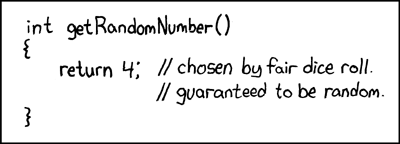
\includegraphics[width=0.4\textwidth]{img/random_number.png}
  \caption{xkcd, source: \url{https://imgs.xkcd.com/comics/random_number.png}, license: CC-BY-NC}
  \label{fig:dilbertRNG}
\end{figure}



A good source of random numbers is essential for many crypto
operations. The key feature of a good random number generator is the
non-predictability of the generated numbers. This means that hardware
support for generating entropy is essential.


Hardware random number generators in operating systems or standalone
components collect entropy from various random events mostly by using
the (low bits of the) time an event occurs as an entropy source. The
entropy is merged into an entropy pool and in some implementations there
is some bookkeeping about the number of random bits available.

\subsection{When random number generators fail}

Random number generators can fail -- returning predictable non-random
numbers -- if not enough entropy is available when random numbers should
be generated.

This typically occurs for embedded devices and virtual machines.
Embedded devices lack some entropy sources other devices have, e.g.:

\begin{itemize*}
  \item No persistent clock, so boot-time is not contributing to the
    initial RNG state
  \item No hard-disk: No entropy from hard-disk timing, no way to store
    entropy between reboots
\end{itemize*}

Virtual machines emulate some hardware components so that the
generated entropy is over-estimated. The most critical component that
has been shown to return wrong results in an emulated environment is the
timing source~\cite{Eng11,POL11}.

Typically the most vulnerable time where low-entropy situations occur is
shortly after a reboot. Unfortunately many operating system installers
create cryptographic keys shortly after a reboot~\cite{HDWH12}.

Another problem is that OpenSSL seeds its internal random generator only
seldomly from the hardware random number generator of the operating
system. This can lead to situations where a daemon that is started at a
time when entropy is low keeps this low-entropy situation for hours
leading to predictable session keys~\cite{HDWH12}.

\subsection{Linux}
\label{subsec:RNG-linux}

%\todo{Other architectures, BSD, Windows?}

On Linux there are two devices that return random bytes when read; the
\verb+/dev/random+ can block until sufficient entropy has been collected
while \verb+/dev/urandom+ will not block and return whatever (possibly
insufficient) entropy has been collected so far.

Unfortunately most crypto implementations are using \verb+/dev/urandom+
and can produce predictable random numbers if not enough entropy has
been collected~\cite{HDWH12}.

Linux supports the injection of additional entropy into the entropy pool
via the device \verb+/dev/random+. On the one hand this is used for
keeping entropy across reboots by storing output of /dev/random into a
file before shutdown and re-injecting the contents during the boot
process. On the other hand this can be used for running a secondary
entropy collector to inject entropy into the kernel entropy pool.

On Linux you can check how much entropy is available with the command:
\begin{lstlisting}
$ cat /proc/sys/kernel/random/entropy_avail
\end{lstlisting}

%% specifics for libraries
%% Openssl uses /dev/urandom. See the paper: https://factorable.net/weakkeys12.conference.pdf (section 5.2)
%% What about other libs? 
%% What about other OSes? 


\subsection{Recommendations}

On Linux, if the \verb+getrandom(2)+ syscall is available, use that instead of reading
from a device file. If \verb+getrandom(2)+ doesn't exist, always read from 
\verb+/dev/urandom+, never \verb+/dev/random+. If you're developing an application that
runs during the system boot or on embededded devices, poll \verb+/dev/random+ until 
it's ready. This will tell you that \verb+/dev/urandom+ has been seeded by the kernel.
Then, feel free to read from \verb+/dev/urandom+. Entropy doesn't run out.

To avoid situations where a newly deployed server doesn't have enough
entropy it is recommended to generate keys (e.g. for SSL or SSH) on
a system with a sufficient amount of entropy available and transfer the generated keys
to the server.  This is especially advisable for small embedded devices
or virtual machines.

For embedded devices and virtual machines deploying additional userspace
software that generates entropy and feeds this to kernel entropy pool
(e.g. by writing to \verb+/dev/random+ on Linux) is recommended. Note
that only a process with root rights can update the entropy counters in the
kernel; non-root or user processes can still feed entropy to the pool but
cannot update the counters~\cite{Wikipedia:/dev/random}.

For Linux the \verb+haveged+
implementation~\cite{HAV13a} based on the HAVEGE~\cite{SS03}
strong random number generator currently looks like the best choice. It
can feed its generated entropy into the kernel entropy pool and recently
has grown a mechanism to monitor the quality of generated random
numbers~\cite{HAV13b}. The memory footprint may be too high for small
embedded devices, though.

For systems where -- during the lifetime of the keys -- it is expected
that low-entropy situations occur, RSA keys should be preferred over DSA
keys: For DSA, if there is ever insufficient entropy at the time keys
are used for signing this may lead to repeated ephemeral keys. An
attacker who can guess an ephemeral private key used in such a signature
can compromise the DSA secret key.
For RSA this can lead to discovery of encrypted plaintext or forged
signatures but not to the compromise of the secret key~\cite{HDWH12}.

\section{Keylengths}
\label{section:keylengths}


\epigraph{``On the choice between AES256 and AES128: I would never consider
using AES256, just like I don't wear a helmet when I sit inside my car. It's
too much bother for the epsilon improvement in security.''}{Vincent Rijmen
in a personal mail exchange Dec 2013}

Recommendations on keylengths need to be adapted regularly. Since this document
first of all is static and second of all, does not consider itself to be
authoritative on keylengths, we would rather refer to existing publications and
websites.  Recommending a safe key length is a hit-and-miss issue.

Furthermore, when choosing an encryption algorithm and key length, the
designer/sysadmin always needs to consider the value of the information and how
long it must be protected.  In other words: consider the number of years the
data needs to stay confidential.


The ECRYPT II publication~\cite{ii2011ecrypt} gives a fascinating overview of
strengths of symmetric keys in chapter 5 and chapter 7. Summarizing ECRYPT II, we
recommend 128 bit of key strength for symmetric keys. In ECRYPT II, this is
considered safe for security level 7, long term protection.

In the same ECRYPT II publication you can find a practical comparison of key size
equivalence between symmetric key sizes and RSA, discrete log (DLOG) and EC
keylengths. ECRYPT II arrives at the interesting conclusion that for an
equivalence of 128 bit symmetric size, you will need to use an 3248 bit RSA
key~\cite[chapter 7, page 30]{ii2011ecrypt}.


There are a couple of other studies comparing keylengths and their respective
strengths.  The website \url{http://www.keylength.com/} compares these papers
and offers a good overview of approximations for key lengths based on
recommendations by different standardization bodies and academic publications.
Figure \ref{fig:keylengths.com} shows a typical comparison of keylengths on
this web site.

\begin{figure}[h]
  \centering
  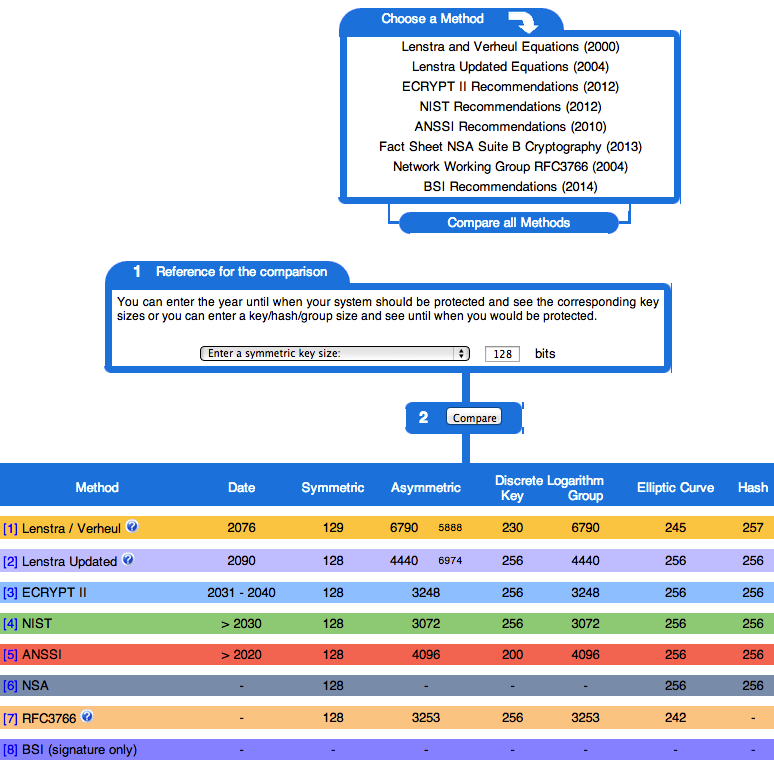
\includegraphics[width=0.65\textwidth]{img/keylengths_com.png}
  \caption{Screenshot of \url{http://www.keylength.com} for 128 bit symmetric key size equivalents}
  \label{fig:keylengths.com}
\end{figure}


\paragraph{Summary}
\begin{itemize*}
  \item For asymmetric public-key cryptography we consider any key length below
3248 bits to be deprecated at the time of this writing (for long term
protection).
  \item For elliptic curve cryptography we consider key lengths below 256 bits to
be inadequate for long term protection.  
  \item For symmetric algorithms we consider anything below 128 bits to be
inadequate for long term protection.
\end{itemize*}

\paragraph{Special remark on 3DES:}
We want to note that 3DES theoretically has 168 bits of security, however based
on the NIST Special Publication 800-57
\footnote{\url{http://csrc.nist.gov/publications/PubsSPs.html\#800-57-part1},
pages 63 and 64}, it is clear that 3DES can only be considered to provide for
80 bits / 112 bits security.

\input{theory/ECC}
\input{theory/SHA}
\input{theory/DH}
\section{Public Key Infrastructures}
\label{section:PKIs}

Public-Key Infrastructures try to solve the problem of verifying
whether a public key belongs to a given entity, so as to prevent Man
In The Middle attacks.

There are two approaches to achieve that: {\it Certificate Authorities}
and the {\it Web of Trust}.

Certificate Authorities (CAs) sign end-entities' certificates, thereby
associating some kind of identity (e.g. a domain name or an email
address) with a public key. CAs are used with TLS and S/MIME
certificates, and the CA system has a big list of possible and real
problems which are summarized in section \ref{sec:hardeningpki} and
\cite{https13}.

The Web of Trust is a decentralized system where people sign each
others keys, so that there is a high chance that there is a ``trust
path'' from one key to another. This is used with PGP keys, and while
it avoids most of the problems of the CA system, it is more
cumbersome.

As alternatives to these public systems, there are two more choices:
running a private CA, and manually trusting keys (as it is used with
SSH keys or manually trusted keys in web browsers).

The first part of this section addresses how to obtain a certificate
in the CA system. The second part offers recommendations on how to
improve the security of your PKI.

\subsection{Certificate Authorities}
\label{sec:cas}
In order to get a certificate, you can find an external CA willing to issue
a certificate for you, run your own CA, or use self-signed certificates.
As always, there are advantages and disadvantages for every one of these
options; a balance of security versus usability needs to be found.

\subsubsection{Certificates From an External Certificate Authority}
\label{sec:signcertfromca}

There is a fairly large number of commercial CAs that will issue
certificates for money.  Some of the most ubiquitous commercial CAs are
Verisign, GoDaddy, and Teletrust.  However, there are also CAs that offer
certificates for free.  The most notable examples are StartSSL, which is a
company that offers some types of certificates for free, and CAcert, which
is a non-profit volunteer-based organization that does not charge at all
for issuing certificates.  Finally, in the research and education field, a
number of CAs exist that are generally well-known and well-accepted within
the higher-education community.

A large number of CAs is pre-installed in client software's or
operating system's``trust stores''; depending on your application, you
have to select your CA according to this, or have a mechanism to
distribute the chosen CA's root certificate to the clients.

When requesting a certificate from a CA, it is vital that you generate the
key pair yourself.  In particular, the private key should never be known to
the CA.  If a CA offers to generate the key pair for you, you should not
trust that CA.

Generating a key pair and a certificate request can be done with a number of
tools.  On Unix-like systems, it is likely that the OpenSSL suite is available
to you.  In this case, you can generate a private key and a corresponding
certificate request as follows:

\begin{lstlisting}
% openssl req -new -nodes -keyout <servername>.key -out <servername>.csr -newkey rsa:<keysize>
Country Name (2 letter code) [AU]:DE
State or Province Name (full name) [Some-State]:Bavaria
Locality Name (eg, city) []:Munich
Organization Name (eg, company) [Internet Widgits Pty Ltd]:Example
Organizational Unit Name (eg, section) []:Example Section
Common Name (e.g. server FQDN or YOUR name) []:example.com
Email Address []:admin@example.com

Please enter the following 'extra' attributes
to be sent with your certificate request
A challenge password []:
An optional company name []:
\end{lstlisting}

\subsubsection{Setting Up Your Own Certificate Authority}
\label{sec:setupownca}
In some situations it is advisable to run your own certificate authority.
Whether this is a good idea depends on the exact circumstances.  Generally
speaking, the more centralized the control of the systems in your
environment, the fewer pains you will have to go through to deploy your own
CA.  On the other hand, running your own CA maximizes the trust level that
you can achieve because it minimizes external trust dependencies.

Again using OpenSSL as an example, you can set up your own CA with the
following commands on a Debian system:

\begin{lstlisting}
% cd /usr/lib/ssl/misc
% sudo ./CA.pl -newca
\end{lstlisting}

Answer the questions according to your setup. Now that you have configured your basic settings and 
issued a new root certificate, you can issue new certificates as follows:

\begin{lstlisting}
% cd /usr/lib/ssl/misc
% sudo ./CA.pl -newreq
\end{lstlisting}

Alternatively, software such as TinyCA\cite{Wikipedia:TinyCA} that
acts as a ``wrapper'' around OpenSSL and tries to make life easier is
available.

\subsubsection{Creating a Self-Signed Certificate}
\label{sec:pki:selfsignedcert}
If the desired trust level is very high and the number of systems involved
is limited, the easiest way to set up a secure environment may be to use
self-signed certificates.  A self-signed certificate is not issued by any
CA at all, but is signed by the entity that it is issued to.  Thus, the
organizational overhead of running a CA is eliminated at the expense of
having to establish all trust relationships between entities manually.

With OpenSSL, a self-signed certificate may be created with this command:

\begin{lstlisting}
% openssl req -new -x509 -key privkey.pem -out cacert.pem -days 1095
\end{lstlisting}

The resulting certificate will by default not be trusted by anyone at all,
so in order to be useful, the certificate will have to be made known a
priori to all parties that may encounter it.


\subsection{Hardening PKI}
\label{sec:hardeningpki}

In recent years several CAs were compromised by attackers in order to get a
hold of trusted certificates for malicious activities. In 2011 the Dutch CA
Diginotar was hacked and all certificates were revoked~\cite{diginotar-hack}.
Recently Google found certificates issued to them, which were not used by the
company~\cite{googlecahack}. The concept of PKIs heavily depends on the
security of CAs.  If they get compromised the whole PKI system will fail. Some
CAs tend to incorrectly issue certificates that were designated to do a
different job than what they were intended to by the CA~\cite{gocode}.

Therefore several security enhancements were introduced by different
organizations and vendors~\cite{tschofenig-webpki}. Currently two
methods are used, DANE~\cite{rfc6698} and Certificate
Pinning~\cite{draft-ietf-websec-key-pinning}. Google recently proposed
a new system to detect malicious CAs and certificates  called Certificate 
Transparency~\cite{certtransparency}.

% \subsubsection{DANE}
% \label{sec:dane}

% \subsubsection{Certificate Pinning}
% \label{sec:certpinning}



% This section deals with settings related to trusting CAs. However,
% our main recommendations for PKIs is: if you are able to run your
% own PKI and disable any other CA, do so. This makes sense most in
% environments where any machine-to-machine communication system
% compatibility with external entities is not an issue.
%% azet: this needs discussion! self-signed certificates simply do not
%% work in practices for real-world scenarios - i.e. websites that
%% actually serve a lot of people

% A good background on PKIs can be found in
% \footnote{\url{https://developer.mozilla.org/en/docs/Introduction_to_Public-Key_Cryptography}}
% \footnote{\url{http://cacr.uwaterloo.ca/hac/about/chap8.pdf}}
% \footnote{\url{http://www.verisign.com.au/repository/tutorial/cryptography/intro1.shtml}}
% .

% \todo{ts: Background and Configuration (EMET) of Certificate Pinning,
%   TLSA integration, When to use self-signed certificates, how to get
%   certificates from public CA authorities (CACert, StartSSL),
%   Best-practices how to create a CA and how to generate private
%   keys/CSRs, Discussion about OCSP and CRLs. TD: Useful Firefox
%   plugins: CipherFox, Conspiracy, Perspectives.}


% ``Certificate Policy''\cite{Wikipedia:Certificate_Policy} (CA)

\section{TLS and its support mechanisms}
\label{section:TLS}
\todo{Add a short intro}

\subsection{HTTP Strict Transport Security (HSTS)}
\label{subsection:HSTS}
%\subsection{HTTP Strict Transport Security}
HTTP Strict Transport Security (HSTS) is a web security policy mechanism. HSTS is realized through HTTP header by which a web server declares that complying user agents (web browsers) should interact with it by using \emph{only} secure HTTPS connections\footnote{\url{https://en.wikipedia.org/wiki/HTTP_Strict_Transport_Security}}. 

HSTS header is bound to a DNS name or domain by which the server was accessed. For example if server serves content for two domains and it is HTTPS enabled only for one domain, the browser won't enforce HSTS for the latter. 

HSTS reduces the risk of active man-in-the-middle attacks such as SSL stripping, and impersonation attacks with \emph{untrusted} certificate. HSTS also helps to avoid unintentional mistakes such as insecure links to a secure web site (missing HTTPS links\footnote{Thus, it might be useful for fixing HTTPS mixed-content related errors, see \url{https://community.qualys.com/blogs/securitylabs/2014/03/19/https-mixed-content-still-the-easiest-way-to-break-ssl}.}), and mistyped HTTPS URLs.  

After the web browser receives a HSTS header in a \emph{correctly}\footnote{Website must load without SSL/TLS browser warnings (certificate is issued by a trusted CA, contains correct DNS name, it is time valid, etc.)} prepared SSL session it will automatically use secure HTTPS links for accessing the server. This prevents unencrypted HTTP access (SSL striping, mistyped HTTPS URLs, etc.) when the server is accessed later by the client. 

When a server (that previously emitted a HSTS header) starts using untrusted certificate, complying user agent must show an error message and \emph{block the server connection}. Thus impersonation MITM attack with \emph{untrusted} certificate cannot occur.

For the initial setup HSTS header needs a trusted secure connection over HTTPS. This limitation can be addressed by compiling a list of STS enabled sites  directly into a browser\footnote{List of the preloaded sites can be found at \url{http://dev.chromium.org/sts}. This list is managed by Google/Chrome but it is also used by Firefox \url{https://wiki.mozilla.org/Privacy/Features/HSTS_Preload_List}}. 

\subsubsection{HSTS Header Directives}
\label{subsubsection:HSTS Header Directives}
HSTS header can be parametrized by two directives:
\begin{itemize*}
  \item max-age=<number-of-seconds> 
	\item includeSubdomains 
\end{itemize*}

\emph{max-age} is a required directive. This directive indicates the number of seconds during which the user agent should enforce the HSTS policy (after the reception of the STS header field from a server).

\emph{includeSubdomains} is an optional directive. This directive indicates that the HSTS Policy applies to this HSTS Host as well as \emph{any subdomains of the host's domain name}.

\subsubsection{HSTS Client Support}
\label{subsubsection:HSTS Client Support}
HSTS is supported\footnote{\url{http://caniuse.com/stricttransportsecurity}} by these web browsers:
\begin{itemize*}
  \item Firefox version >= v4.0
	\item Chrome version >= 4.0
	\item Android Browser >=4.4
	\item Opera version >= 12.0 
	\item Opera mobile >= 16.0
	\item Safari >= 7.0
	\item Microsoft Internet Explorer >= 11 (with update provided 09. June 2015)
	\item Microsoft Edge >= 12
\end{itemize*}

\subsubsection{HSTS Considerations}
\label{subsubsection:HSTS Considerations}
Before enabling HSTS it is recommended to consider following:
\begin{itemize*}
  \item Is it \emph{required} to serve content or services over HTTP?
	\item Enabling \emph{includeSubdomains} and SSL certificate management.
	\item Proper value of \emph{max-age}. 
\end{itemize*}

It is recommended to serve all content using HTTPS, but there are exceptions to this rule as well. Consider running a private PKI\footnote{see \nameref{section:PKIs}}. CRLs and OCSP responses are published typically by HTTP protocol. If HSTS is enabled on the site where OCSP and CRLs are published the browser might fail fetching CRL or validating OCSP response.

Similar reasoning goes for \emph{includeSubdomains}. One needs to be sure that HTTPS can be enforced for all subdomains. Moreover the administrators are advised to watch for expiration of the SSL certificate and handle the renewal process with caution. If a SSL certificate is renewed after expiration or misses a (HSTS enabled) domain name, the connection to site will break (without providing override mechanism to the end user).  

Finally HSTS should be tested with lower \emph{max-age} values and deployed with higher \emph{max-age} values. 

\subsubsection{Testing HSTS}
\label{subsubsection:Testing HSTS}
HSTS can be tested either using locally or through the Internet. 

For local testing it is possible to utilize Chrome Web browser UI by typing \url{chrome://net-internals/#hsts}\footnote{see \url{http://blog.chromium.org/2011/06/new-chromium-security-features-june.html}} in the address bar.

Testing over the Internet can be conducted by Qualys SSL Labs test \url{https://www.ssllabs.com/ssltest/}. \emph{Strict Transport Security (HSTS)} information is located in the \emph{Protocol Details} section.

\subsubsection{References}
\begin{itemize*}
	\item Websites Must Use HSTS in Order to Be Secure \url{https://www.eff.org/deeplinks/2014/02/websites-hsts}
	\item OWASP: HTTP Strict Transport Security: \url{https://www.owasp.org/index.php/HTTP_Strict_Transport_Security}
	\item HSTS Browser Compatibility List: \url{http://caniuse.com/stricttransportsecurity}
  \item RFC 6797:HTTP Strict Transport Security (HSTS) - Examples: \url{https://tools.ietf.org/html/rfc6797#section-6.2}
\end{itemize*}




\subsection{HTTP Public Key Pinning (HPKP)}
\label{subsection:HPKP}
%\subsection{HTTP Public Key Pinning (HPKP)}
Much like HTTP Strict Transport Security (HSTS), HTTP Public Key Pinning (HPKP) is a Trust On First Use (TOFU) mechanism. It protects HTTPS websites from impersonation using certificates issued by compromised certificate authorities. The data for Pinning is supplied by an HTTP-Header sent by the WebServer. 

\subsubsection{HPKP Header Directives}
\label{subsubsection:HPKP Header Directives}
HPKP provides two different types of headers:
\begin{itemize*}
  \item Public-Key-Pins
	\item Public-Key-Pins-Report-Only
\end{itemize*}
HPKP header can be parametrized by following directives:
\begin{itemize*}
  \item pin-sha256="<YOUR\_PUBLICKEY\_HASH=>"
  \item max-age=<number-of-seconds> 
	\item includeSubdomains 
	\item report-uri="<https://YOUR.URL/TO-REPORT>"
\end{itemize*}

\textbf{pin-sha256} is a required directive. It can and should be used several (at least two) times for specifying the public keys of your domain-certificates or CA-certificates. Operators can pin any one or more of the public keys in the certificate-chain, and indeed must pin to issuers not in the chain (as, for example, a Backup Pin). Pinning to an intermediate issuer, or even to a trust anchor or root, still significantly reduces the number of issuers who can issue end-entity certificates for the Known Pinned Host, while still giving that host flexibility to change keys without a disruption of service. OpenSSL can be used to convert the Public Key of an X509-Certificate as follows:
\begin{lstlisting}
openssl x509 -in <certificate.cer> -pubkey -noout | 
 openssl rsa -pubin -outform der | 
 openssl dgst -sha256 -binary | 
 openssl enc -base64
writing RSA key
pG3WsstDsfMkRdF3hBClXRKYxxKUJIOu8DwabG8MFrU=
\end{lstlisting} 
This piped usage of OpenSSL first gets the Public-Key of <certificate.cer>, converts it do DER (binary) format, calculates an SHA256 Hash and finally encodes it Base64. The output (including the ending Equal-Sign) is exactly whats needed for the \emph{pin-sha256="<YOUR\_PUBLICKEY\_HASH=>"} parameter. To generate the Hash for a prepared Backup-Key just create a Certificate-Signing-Request and replace "\texttt{openssl x509}" by "\texttt{openssl req -in <backup-cert.csr> -pubkey -noout}" as first OpenSSL command.\\ 
Instead of using OpenSSL even WebServices like \url{https://report-uri.io/home/pkp_hash/} can be used to get a suggestion for the possible Public-Key-Hashes for a given WebSite.

\textbf{max-age} is a required directive (when using the \emph{Public-Key-Pins} header). This directive specifies the number of seconds during which the user agent should regard the host (from whom the message was received) as a Known Pinned Host.

\textbf{includeSubdomains} is an optional directive. This directive indicates that the same pinning applies to this Host as well as \emph{any subdomains of the host's domain name}. Be careful - you need to use a Multi-Domain/Wildcard-Certificate or use the same Pub/Private-Keypair in all Subdomain-Certificates or need to pin to CA-Certificates signing all your Subdomain-Certificates.

\textbf{report-uri} is an optional directive. The presence of a report-uri directive indicates to the Browser that in the event of Pin Validation failure it should post a report to the report-uri (HTTP-Post is done using JSON, Syntax see {RFC-7469 Section 3}\footnote{\url{https://tools.ietf.org/html/rfc7469\#section-3}}). There are WebServices like \url{https://report-uri.io/} out there which can be used to easily collect and visualize these reports.

\subsubsection{HPKP Client Support}
\label{subsubsection:HPKP Client Support}
HPKP is supported\footnote{\url{http://caniuse.com/\#feat=publickeypinning}} by these web browsers:
\begin{itemize*}
  \item Firefox version >= 35
	\item Chrome version >= 38
	\item Android Browser >= 44
	\item Opera version >= 25 
\end{itemize*}
Currently (16. Oct 2015) there is no HPKP Support in: Apple Safari, Microsoft Internet Explorer and Edge.

\subsubsection{HPKP Considerations}
\label{subsubsection:HPKP Considerations}
Before enabling HPKP it is recommended to consider following:
\begin{itemize*}
  \item Which Public-Keys to use for Pinning (Certificat + Backup-Certificate, CAs, Intermediate-CAs)
	\item Proper value of \emph{max-age}. Start testing with a short Period, increase Period after deployment.
	\item Be careful when using \emph{includeSubdomains}, are all your subdomains covered by the defined Public-Key-Hashes?
\end{itemize*}

The administrators are advised to watch for expiration of the SSL certificate and handle the renewal process with caution. If a SSL certificate is renewed without keeping the Public-Key (reusing the CSR) for an HPKP enabled domain name, the connection to site will break (without providing override mechanism to the end user).  

\subsubsection{Testing HPKP}
\label{subsubsection:Testing HPKP}
HPKP can be tested either using locally or through the Internet. 

There is a handy Bash-Script which uses OpenSSL for doing several SSL/TLS-Tests available at \url{https://testssl.sh/}
\begin{lstlisting}
wget -q https://testssl.sh/testssl.sh
wget -q https://testssl.sh/mapping-rfc.txt
chmod 755 ./testssl.sh
./testssl.sh https://your-domain.com

# Sample Output, just HSTS and HPKP Section (Full report is quite long!):
Strict Transport Security    182 days=15724800 s, includeSubDomains
Public Key Pinning # of keys: 2, 90 days=7776000 s, just this domain
           matching host key: pG3WsstDsfMkRdF3hBClXRKYxxKUJIOu8DwabG8MFrU
\end{lstlisting}

For local testing it is possible to utilize Google Chrome Web browser, just open the Chrome net-internals-URL: \url{chrome://net-internals/#hsts}.

For Mozilla Firefox there is an Plug-In provided by the "Secure Information Technology Center Austria" available: \url{https://demo.a-sit.at/firefox-plugin-highlighting-safety-information/}

Testing over the Internet can be conducted by Qualys SSL Labs test \url{https://www.ssllabs.com/ssltest/}. \emph{Public Key Pinning (HPKP)} information is located in the \emph{Protocol Details} section. 

There is also a fast online HPKP-only check at \url{https://report-uri.io/home/pkp_analyse}.

\subsubsection{References}
\begin{itemize*}
	\item OWASP: Certificate and Public Key Pinning: \url{https://www.owasp.org/index.php/Certificate_and_Public_Key_Pinning}
	\item HPKP Browser Compatibility List: \url{http://caniuse.com/\#feat=publickeypinning}
  \item RFC 7469:Public Key Pinning Extension for HTTP - Examples: \url{https://tools.ietf.org/html/rfc7469\#section-2.1.5}
\end{itemize*}




%\subsection{Server Name Indication}
\chapter{Appendix}
\chapter{Tools}
\label{cha:tools}
This section lists tools for checking the security settings.

\section{SSL \& TLS}

Server checks via the web
\begin{itemize*}
  \item \href{https://ssllabs.com}{ssllabs.com} offers a great way to check your webserver for misconfigurations. See \url{https://www.ssllabs.com/ssltest/}. Furthermore, ssllabs.com has a good best practices tutorial, which focuses on avoiding the most common mistakes in SSL.
  \item SSL Server certificate installation issues \url{https://www.sslshopper.com/ssl-checker.html}
  \item Check SPDY protocol support and basic TLS setup \url{http://spdycheck.org/}
  \item XMPP/Jabber Server check (Client-to-Server and Server-to-Server) \url{https://xmpp.net/}
  \item Luxsci SMTP TLS Checker \url{https://luxsci.com/extranet/tlschecker.html}
  \item Does your mail server support StartTLS? \url{https://starttls.info/}
  \item \url{http://checktls.com} is a tool for testing arbitrary TLS services.
  \item \url{http://tls.secg.org} is a tool for testing interoperability of HTTPS implementations for ECC cipher suites.
  \item \url{http://www.whynopadlock.com/} Testing for mixed SSL parts loaded via http that can totally lever your HTTPS.
\end{itemize*}

Browser checks
\begin{itemize*}
  \item Check your browser's SSL capabilities: \url{https://cc.dcsec.uni-hannover.de/} and \url{https://www.ssllabs.com/ssltest/viewMyClient.html}.
  \item Check Browsers SSL/TLS support and vulnerability to attacks: \url{https://www.howsmyssl.com}
\end{itemize*}


Command line tools
\begin{itemize*}
  \item \url{https://sourceforge.net/projects/sslscan} connects to a given SSL service and shows the cipher suites that are offered.
  \item \url{http://www.bolet.org/TestSSLServer/} tests for BEAST and CRIME vulnerabilities.
  \item \url{https://github.com/drwetter/testssl.sh} checks a server's service on any port for the support of TLS/SSL ciphers, protocols as well as some cryptographic flaws (CRIME, BREACH, CCS, Heartbleed).
  \item \url{https://github.com/iSECPartners/sslyze} Fast and full-featured SSL scanner
  \item \url{https://github.com/jvehent/cipherscan} Fast TLS scanner (ciphers, order, protocols, key size and more)
  \item \url{http://nmap.org/} nmap security scanner
  \item \url{http://www.openssl.net} OpenSSL s\_client
\end{itemize*}


\section{Key length}
\begin{itemize*}
  \item \url{http://www.keylength.com} comprehensive online resource for comparison of key lengths according to common recommendations and standards in cryptography.
\end{itemize*}


\section{RNGs}

%% NOTE: should we merge that with chapter 6.6??
\begin{itemize*}
  \item \href{http://www.fourmilab.ch/random/}{ENT} is a pseudo random number generator sequence tester.
  \item \href{http://www.phy.duke.edu/~rgb/General/dieharder.php}{Dieharder} a random number generator testing tool.
  \item \href{http://www.cacert.at/random/}{CAcert Random} another random number generator testing service.
\end{itemize*}

\section{Guides}
\begin{itemize*}
  \item See: \url{https://www.ssllabs.com/downloads/SSL_TLS_Deployment_Best_Practices.pdf}.
\end{itemize*}

\chapter{Links}
\label{cha:links}
%% NOTE: this should re restructured...

\begin{itemize*}
  \item IANA official list of Transport Layer Security (TLS) Parameters: \url{https://www.iana.org/assignments/tls-parameters/tls-parameters.txt}
  \item SSL cipher settings: \url{http://www.skytale.net/blog/archives/22-SSL-cipher-setting.html}
  \item Elliptic curves and their implementation (04 Dec 2010): \url{https://www.imperialviolet.org/2010/12/04/ecc.html}
  \item A (relatively easy to understand) primer on elliptic curve cryptography: \url{http://arstechnica.com/security/2013/10/a-relatively-easy-to-understand-primer-on-elliptic-curve-cryptography}
  \item Duraconf, A collection of hardened configuration files for SSL/TLS services (Jacob Appelbaum's github): \url{https://github.com/ioerror/duraconf}
  \item Attacks on SSL a comprehensive study of BEAST, CRIME, TIME, BREACH, LUCKY 13 \& RC4 Biases: \url{https://www.isecpartners.com/media/106031/ssl_attacks_survey.pdf}
  \item EFF How to deploy HTTPS correctly: \url{https://www.eff.org/https-everywhere/deploying-https}
  \item Bruce Almighty: Schneier preaches security to Linux faithful (on not recommending to use Blowfish anymore in favor of Twofish): \url{https://www.computerworld.com.au/article/46254/bruce_almighty_schneier_preaches_security_linux_faithful/?pp=3}
  \item Implement FIPS 183-3 for DSA keys (1024bit constraint): \url{https://bugzilla.mindrot.org/show_bug.cgi?id=1647}
  \item Elliptic Curve Cryptography in Practice: \url{http://eprint.iacr.org/2013/734.pdf}
  \item Factoring as a Service: \url{http://crypto.2013.rump.cr.yp.to/981774ce07e51813fd4466612a78601b.pdf}
  \item Black Ops of TCP/IP 2012: \url{http://dankaminsky.com/2012/08/06/bo2012/}
  \item SSL and the Future of Authenticity, Moxie Marlinspike - Black Hat USA 2011: \url{https://www.youtube.com/watch?v=Z7Wl2FW2TcA}
  \item ENISA - Algorithms, Key Sizes and Parameters Report (Oct.'13) \url{http://www.enisa.europa.eu/activities/identity-and-trust/library/deliverables/algorithms-key-sizes-and-parameters-report}
  \item Diffie-Hellman Groups \url{http://ibm.co/18lslZf}
  \item Diffie-Hellman Groups standardized in RFC3526~\cite{rfc3526} \url{https://datatracker.ietf.org/doc/rfc3526/}
  \item ECC-enabled GnuPG per RFC6637~\cite{rfc6637} \url{https://code.google.com/p/gnupg-ecc}
  \item TLS Security (Survey + Lucky13 + RC4 Attack) by Kenny Paterson \url{https://www.cosic.esat.kuleuven.be/ecc2013/files/kenny.pdf}
  \item Ensuring High-Quality Randomness in Cryptographic Key Generation \url{http://arxiv.org/abs/1309.7366v1}
  \item Wikipedia: Ciphertext Stealing \url{https://en.wikipedia.org/wiki/Ciphertext_stealing}
  \item Wikipedia: Malleability (Cryptography) \url{https://en.wikipedia.org/wiki/Malleability_(cryptography)}
  \item Ritter's Crypto Glossary and Dictionary of Technical Cryptography \url{http://www.ciphersbyritter.com/GLOSSARY.HTM}
\end{itemize*}

\chapter{Suggested Reading}
\label{cha:suggested-reading}
This section contains suggested reading material.

\begin{itemize*}
	\item Cryptography Engineering: Design Principles and Practical Applications, Ferguson, N. and Schneier, B. and Kohno, T. (ISBN-13: 978-0470474242)
	\item Security Engineering: A Guide to Building Dependable Distributed Systems, Anderson, R.J. (ISBN-13: 978-0470068526)
	\item Applied cryptography: protocols, algorithms, and source code in C, Schneier, B. (ISBN-13: 978-0471117094)
	\item Guide to Elliptic Curve Cryptography, Hankerson, D. and Vanstone, S. and Menezes, A.J. (ISBN-13: 978-0387952734)
	\item A Introduction To The Theory of Numbers, Godfrey Harold Hardy, E. M. Wrigh (ISBN-13: 978-0199219865)
	\item Malicious Cryptography: Exposing Cryptovirology, Young A., Yung, M. (ISBN-13: 978-0764549755)
\end{itemize*}

%% should we include bibtex instead? can be downloaded from books.google.com

\input{cipher_suite_names}
\chapter{Further research}
\label{cha:further-research}
The following is a list of services, software packages, hardware devices or protocols that we considered documenting but either did not manage to document yet or might be able to document later. We encourage input from the Internet community. 

\begin{multicols}{3}
\begin{itemize*}
  \item whatsapp (might be problematic since a user/admin can't change anything)
  \item Lync
  \item Skype (might be problematic since a user/admin can't change anything)
  \item Wi-Fi APs, 802.1X
  \item Tomcat
  \item SIP
  \item SRTP
  \item DNSSec (mention BCPs)
  \item DANE
  \item TOR
  \item S/Mime (check are there any BCPs? )
  \item TrueCrypt, LUKS, FileVault
  \item AFS
  \item Kerberos
  \item NNTP
  \item NTPs tlsdate
  \item BGP / OSPF
  \item SILC
  \item LDAP
  \item seclayer-tcp
  \item Commerical network equipment vendors
  \item RADIUS
  \item Moxa , APC, und co... ICS . Ethernet to serial
  \item telnet (only sensible recommendation: \emph{DON't!!})
  \item rsyslog
  \item v6 spoofing (look at work by Ferndo Gont, Marc Heuse, et. al.)
  \item tinc
  \item racoon
  \item l2tp
  \item rsync
  \item telnets
  \item ftps
  \item webmin (probably the same recommendations as with Apache apply, but where does that need to be configured?)
  \item plesk (same as webmin)
  \item phpmyadmin (same as webmin)
  \item DSL modems (where to start?)
  \item UPnP, natPmp
  \item SAML federated auth providers \footnote{e.g., all the REFEDS folks (\url{https://refeds.org/})), including InCommon (\url{http://www.incommon.org/federation/metadata.html}
  \url{https://wiki.shibboleth.net/confluence/display/SHIB2/TrustManagement} }
  \item Microsoft SQL Server
\end{itemize*}
\end{multicols}

%%% Local Variables: 
%%% mode: latex
%%% TeX-master: "applied-crypto-hardening"
%%% End: 

%\newpage
\section{Reviewers}
\label{section:Reviewers}

We would like to express our thanks to the following reviewers (in alphabetical order):


\vline{}

\begin{minipage}[b]{0.5\linewidth}
\center
Brown, Scott \\
Gühring Philipp  \\
Grigg, Ian  \\
Horenbeck, Maarten \\
Kovacic, Daniel \\
Lenzhofer, Stefan \\
\end{minipage}
\begin{minipage}[b]{0.5\linewidth}
\center
Mendel, Florian \\
Millauer, Tobias \\
Pichler, Patrick \\
Pöschl, Ulrich \\
San, Berg \\
Schreck, Thomas  \\
Wagner, Sebastian («sebix») \\
\end{minipage}


%% *@discuss@lists.cert.at --> AKA
%% devops mailing lists --> Pepi, Azet
%% cryptography liste (at release time) --> Azet



\input{bib}

\end{document}
